\documentclass[10pt]{beamer}

\usetheme{metropolis}
\usecolortheme{beaver}
\usepackage{appendixnumberbeamer}

\usepackage{booktabs}
\usepackage[scale=2]{ccicons}

\usepackage{pgfplots}
\usepgfplotslibrary{dateplot}

\usepackage{xspace}
\newcommand{\themename}{\textbf{\textsc{metropolis}}\xspace}
\usepackage[brazil]{babel}  % AAB
\usepackage{bibentry}         % AAB
%\usepackage[round,sort,nonamebreak]{natbib}
%\usepackage{natbib}
%
\DeclareMathOperator{\traco}{tr} %AAB
\graphicspath{{../Dissertacao/figuras/}}        % AAB - caminho das figuras (recomendável) 

\title{Fusão de evidências na detecção de bordas em imagens PolSAR}
%\subtitle{A modern beamer theme}
\date{\today}
\author{Anderson Adaime de Borba\\
        Orientador: Dr. Mauricio Marengoni - UPM\\
        Coorientador: Dr. Alejandro Frery - UFAL} 
\institute{Exame de Qualificação - 2018 \\
PPGEEC - Programa de Pós graduação em Engenharia Elétrica e Computação\\
UPM - Universidade Presbiteriana Mackenzie}
\titlegraphic{\hfill
\includegraphics[height=1.1cm]{logo_mack1.pdf}}

\begin{document}

\maketitle

\begin{frame}{Cronograma}
  \setbeamertemplate{section in toc}[sections numbered]
  \tableofcontents[hideallsubsections]
\end{frame}

\section{Introdução}

\begin{frame}[fragile]{Imagens PolSAR}
\textit{Polarimetric Synthetic Aperture Radar} - PolSAR
\begin{alertblock}{Características das imagens PolSAR}
\begin{itemize}
\item Podem estar em plataformas elevadas, aeronaves tripuladas ou não, satélites orbitando a terra ou outros planetas;
\item É uma técnica de produção de imagem viável e prática;
\item Possui alta resolução;
\item Os radares produzem imagens dia e noite;
\item O clima não interfere na captação de imagens.
\end{itemize}
\end{alertblock}

  
\end{frame}
\begin{frame}[fragile]{Imagens PolSAR}
\begin{alertblock}{Aplicações das imagens PolSAR}
  \begin{itemize}
\item Sensoriamento remoto;
\item Topografia;
\item Oceanografia;
\item Glaciologia;
\item Agricultura;
\item Geologia;
\item Florestas;
\item Alvos fixos ou em movimento;
\item Monitoramento ambiental;
\item Controle de derramamento de petróleo;
\item E no auxílio de sistemas óticos.
\end{itemize}
\end{alertblock}
\end{frame}

%\section{Title format}

\begin{frame}{Imagem da baía de San Franscisco}
	\begin{figure}[hbt]
\minipage{0.35\textwidth}
  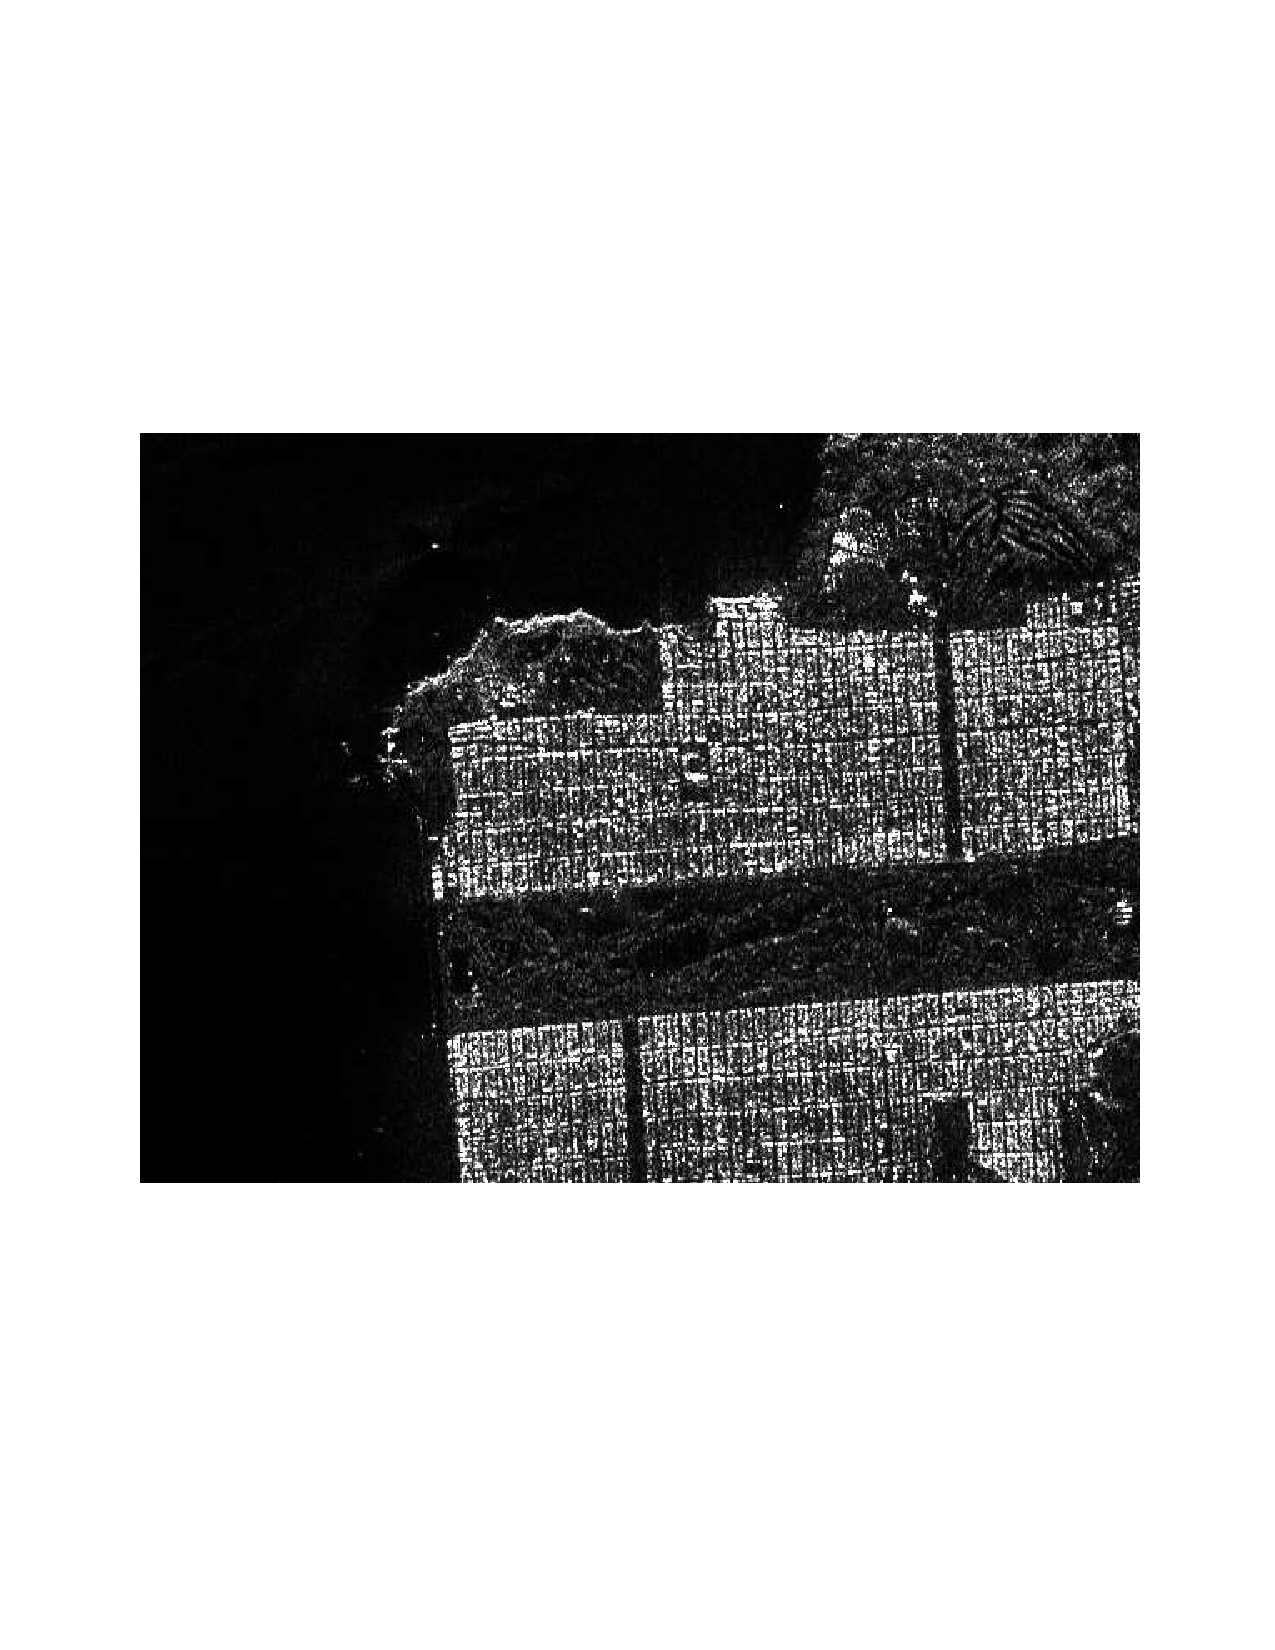
\includegraphics[width=\linewidth]{sf_hh.pdf}
\endminipage
\minipage{0.35\textwidth}
	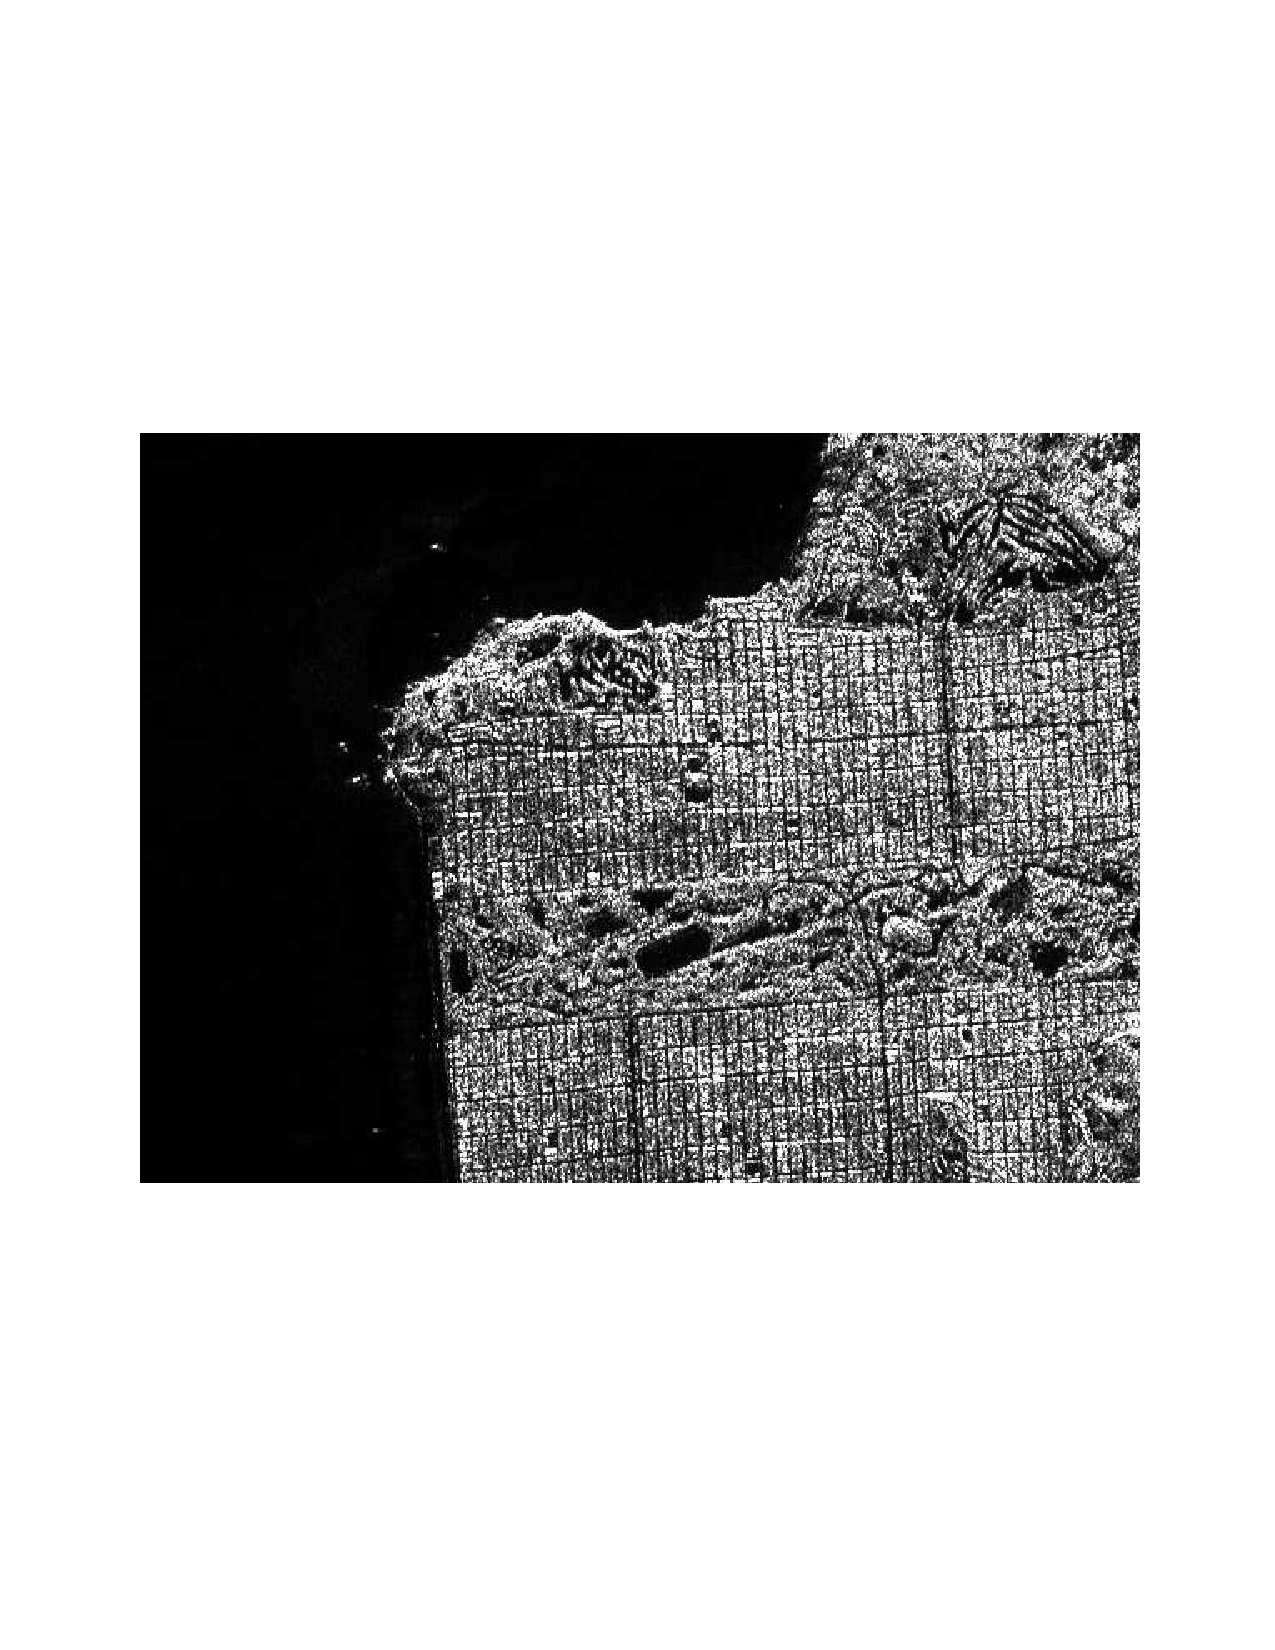
\includegraphics[width=\linewidth]{sf_vh.pdf}
\endminipage
%\centering
\minipage{0.35\textwidth}
	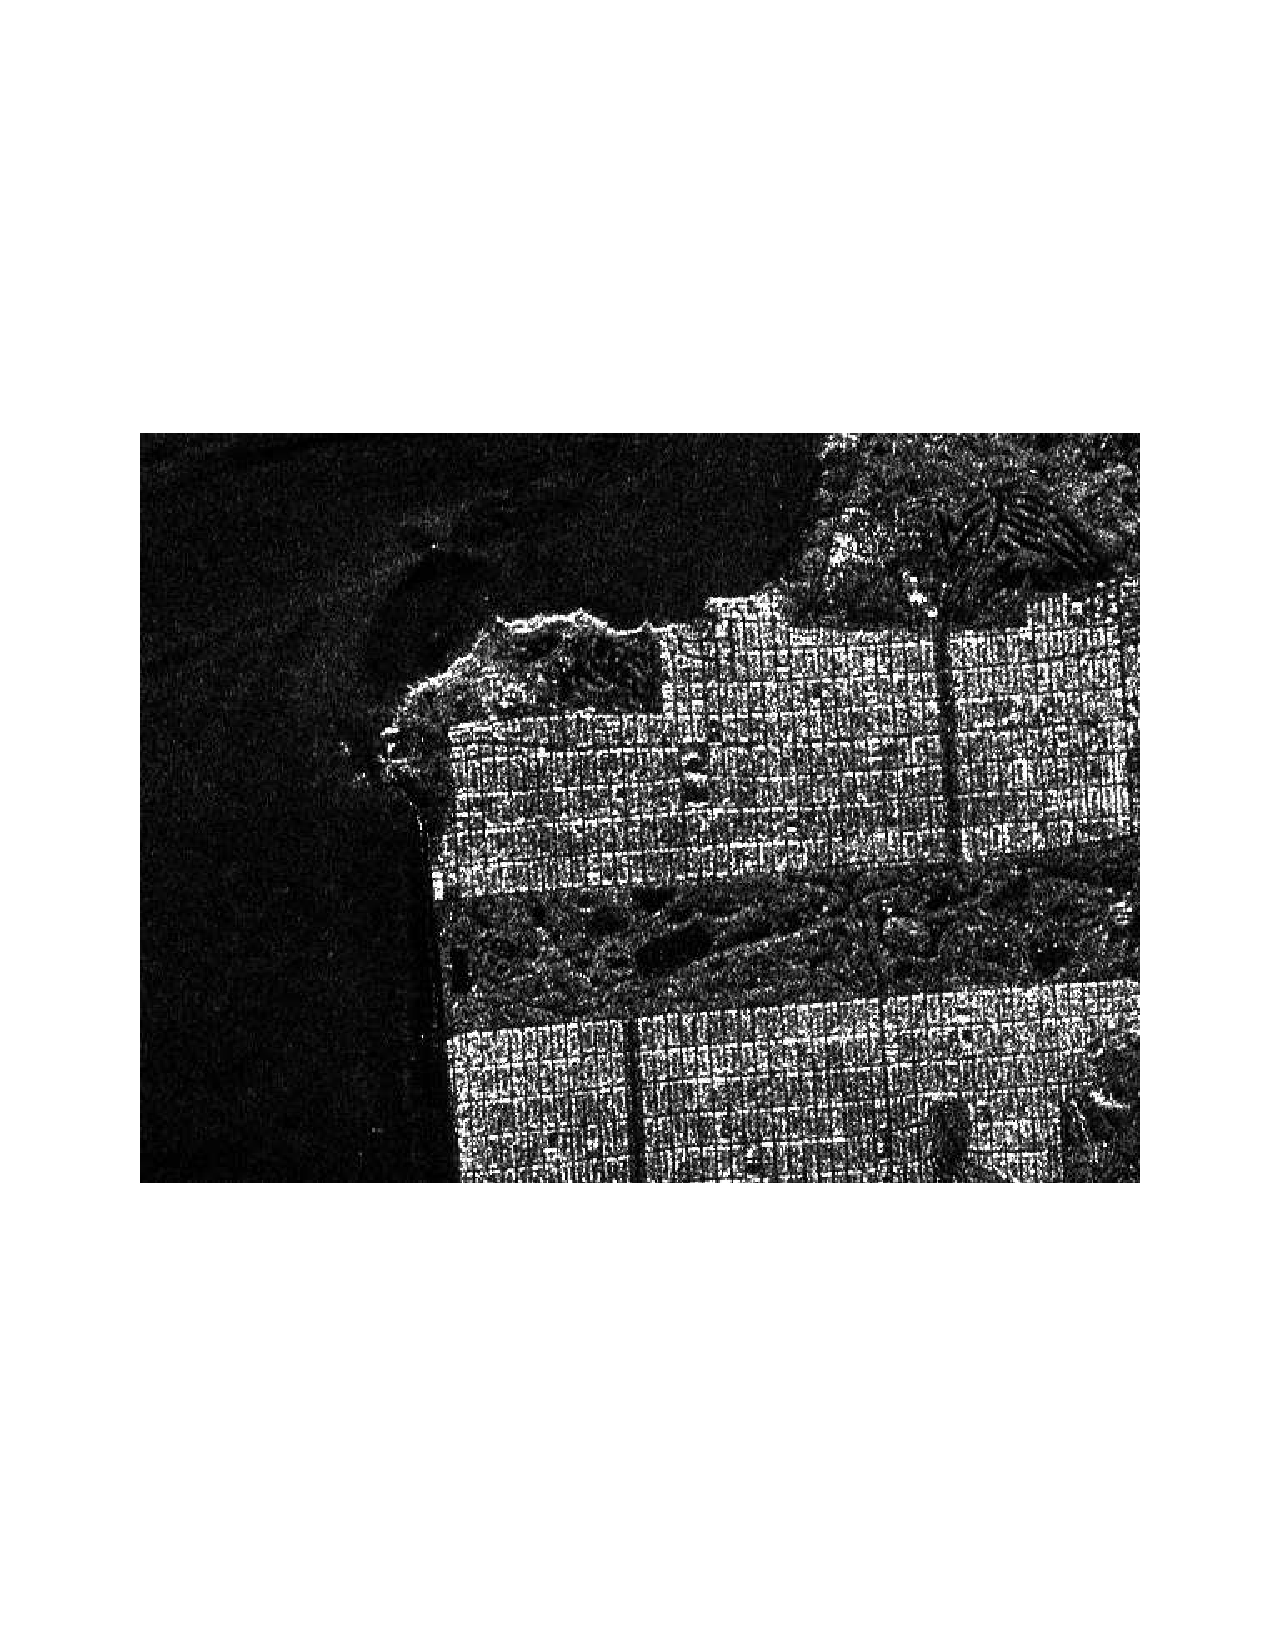
\includegraphics[width=\linewidth]{sf_vv.pdf}
\endminipage
  %      \vspace{-2.0cm}
	\caption{Imagem PolSAR com polarizações ($hh$, $hv$ e $vv$).}
\end{figure}
\end{frame}

\begin{frame}{Imagem da baía de San Franscisco}
\begin{figure}[hbt]
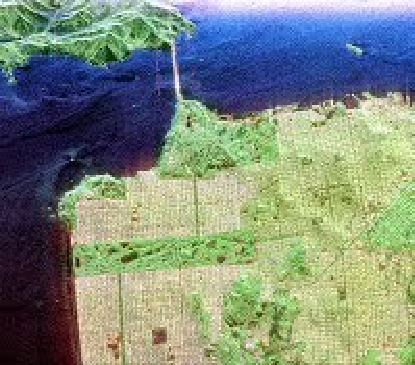
\includegraphics[scale=0.85]{polsar_teste.pdf}
\caption{Baía de São Francisco.}
\end{figure}
\end{frame}

\section{Metodologia}
\begin{frame}{Modelagem estatística para dados PolSAR}
	
\begin{alertblock}{Equação de espalhamento}
\begin{equation}
 \left[
\begin{array}{c}
	E_{h}^{r}   \\
	E_{v}^{r}    \\
\end{array}
\right]
 = \frac{e^{\hat{\imath} kr}}{r}\left[
\begin{array}{cc}
	S_{hh}   & S_{hv}   \\
	S_{vh}   & S_{vv}   \\
\end{array}
\right]
 \left[
\begin{array}{c}
	E_{h}^{t}   \\
	E_{v}^{t}    \\
\end{array}
\right]
\end{equation}
\end{alertblock}
\begin{itemize}
	\item \alert{ $E_{i}^{j}$ - onda eletromagnética;}
	\item \alert{ $h$ - subíndice indicando polarização na direção horizontal;}
	\item \alert{ $v$ - subíndice indicando polarização na direção vertical;}
	\item \alert{ $t$ - superíndice indicando onda transmitida;}
	\item \alert{ $r$ - superíndice indicando onda recebida;}
	\item \alert{ $k$ - número de onda;}
	\item \alert{ $r$ - distância entre radar e alvo.}
\end{itemize}
\end{frame}

\begin{frame}{Modelagem estatística para dados PolSAR}
	\begin{alertblock}{Matriz Hermitiana}
	\begin{itemize}
	\item Matriz de espalhamento
	\begin{equation}
\mathbf{S} = \left[
\begin{array}{cc}
	S_{hh}   & S_{hv}   \\
	S_{vh}   & S_{vv}   \\
\end{array}
\right],
\end{equation}
\alert{ $S_{ij}$ - Coeficiente de espalhamento, $i$ representa o índice do recebimento, e $j$ representa o índice da transmissão da onda.}
\item Teorema da reciprocidade: As propriedades de transmissão e recebimento de uma antena são idênticas, então $S_{hv}=S_{vh}$,
\begin{equation}
\mathbf{s} = \left[
\begin{array}{c}
	S_{hh}      \\
    S_{vh}     \\
	S_{vv}      \\
\end{array}
\right].
\end{equation}
\end{itemize}
\end{alertblock}
\end{frame}

\begin{frame}[fragile]{Modelagem estatística para dados PolSAR}
      
  \alert{Função de probabilidade para distribuição Wishart} 
%
\begin{equation}
    f_{\mathbf{Z}}(\mathbf{Z};\Sigma,L)=\frac{L^{mL}|\mathbf{Z}|^{L-m}}{|\Sigma|^{L}\Gamma_m(L)} \exp(-L\traco{(\Sigma^{-1}\mathbf{Z})}), 
\end{equation}
    \alert{$\Gamma_m(L)$ - Função Gamma multivariada}
\begin{equation}
	\Gamma_m(L)=\pi^{\frac{1}{2}m(m-1)} \prod_{i=0}^{m-1}\Gamma(L-i).
\end{equation}
\end{frame}

\begin{frame}[fragile]{Modelagem estatística para dados PolSAR}
\begin{alertblock}{Aplicações das imagens PolSAR, \cite{of}}
  \begin{itemize}
\item seja a matriz de covariância $\Sigma_{3\times 3}$;
\item fatoração de Cholesky (Fatoração de Crout) $\Sigma= CC^{H}$;
\item gerar um vetor $\mathbf{s_i}_{3\times 1}= C\mathbf{W_i}_{3\times 1}$;
\item onde $\mathbf{W_i}$ é distribuído como uma distribuição normal multivariada com média zero;
\item definindo ;
\begin{equation}
\begin{array}{ccc}
    B&=&\displaystyle{\sum_{i=1}^{NA} {\mathbf{W}_i}{\mathbf{W}_i}^H}, \\
\end{array}
\end{equation}
\item no caso $NA=800*800$;
\item o número de visadas $L$ é usado na multiplicação $\mathbf{W}_i\mathbf{W}_i^H$.
\end{itemize}
\end{alertblock}
\end{frame}

\begin{frame}[fragile]{Modelagem estatística para dados PolSAR}
\begin{alertblock}{Aplicações das imagens PolSAR}
  \begin{itemize}
\item Portanto;
\begin{equation}
\begin{array}{ccc}
    B&=&\displaystyle{\sum_{i=1}^{NA} \mathbf{W}_i\mathbf{W}_i^H}, \\
\end{array}
\end{equation}
\begin{equation}
\begin{array}{ccc}
    CBC^H&=&\displaystyle{\sum_{i=1}^{NA} C\mathbf{W}_i\mathbf{W}_i^HC^H}, \\
\end{array}
\end{equation}
\begin{equation}
\begin{array}{ccc}
    CBC^H&=&\displaystyle{\sum_{i=1}^{NA} C\mathbf{W}_i(C\mathbf{W}_i)^H}. \\
\end{array}
\end{equation}
\item logo;
\end{itemize}
\end{alertblock}
      \alert{Matriz de covariância amostral estimada {\bf Z}}
\begin{equation}
\begin{array}{ccc}
    \mathbf{Z}&=&\displaystyle{\sum_{i=1}^{NA} {\mathbf{s}_i}{\mathbf{s}_i}^H}. \\
\end{array}
\end{equation}
\end{frame}

\begin{frame}{Detecção de bordas em imagens PolSAR}
  \begin{figure}[hbt]
\centering
	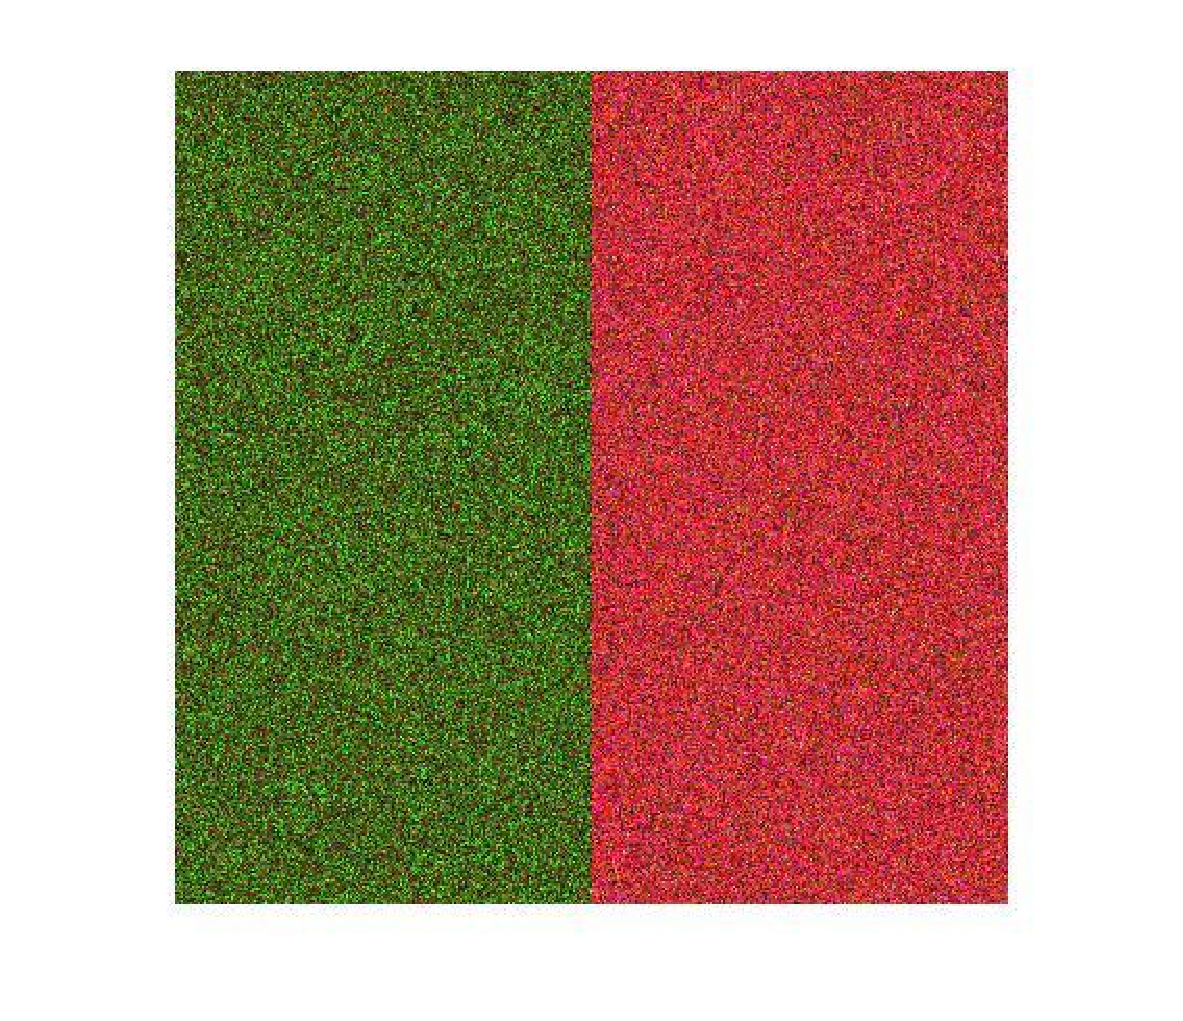
\includegraphics[scale=0.4]{phanton_nhfc_dec_pauli.pdf}
	\caption{Decomposição de Pauli para a phantom.}
\end{figure}
\end{frame}


\begin{frame}{Detecção de bordas em imagens PolSAR}
\begin{figure}[hbt]
	\centering
	%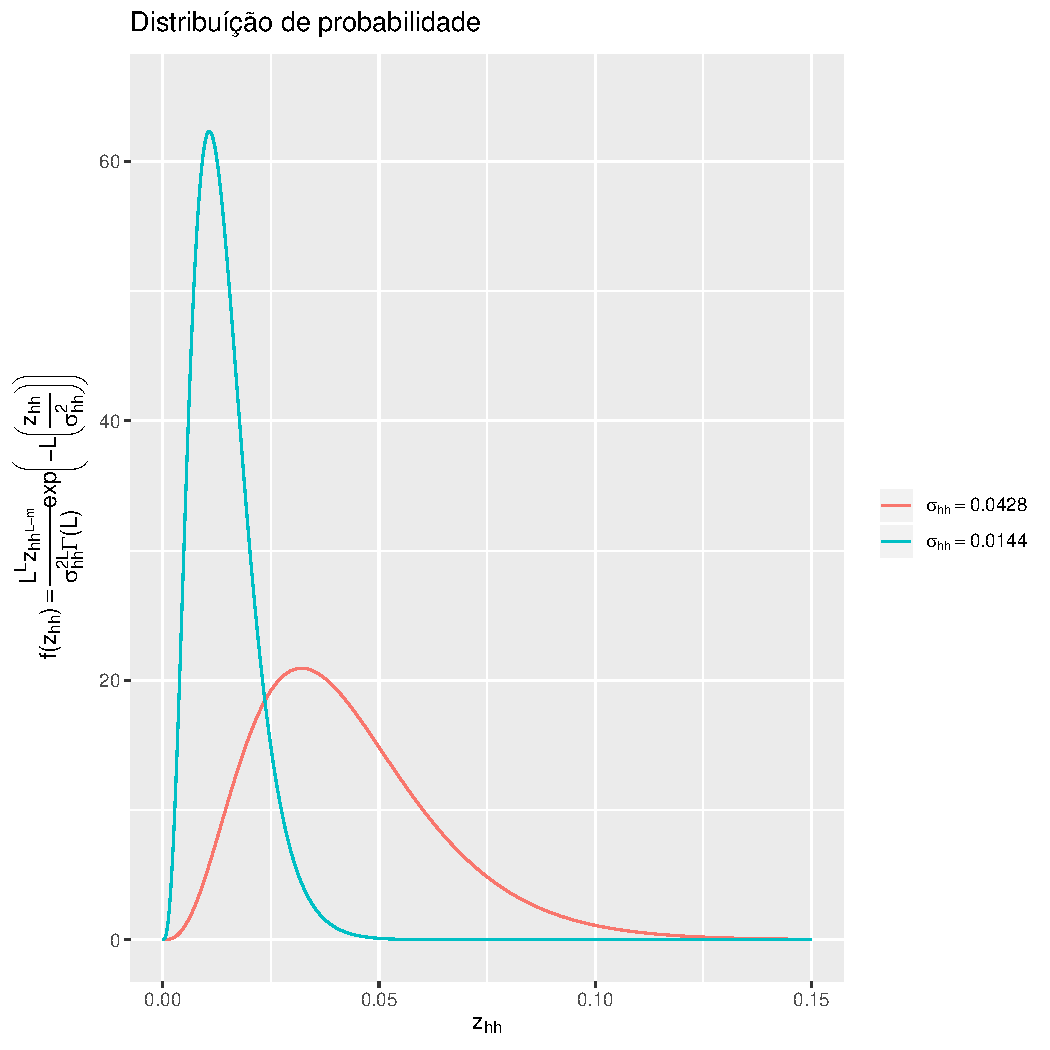
\includegraphics[scale = 1]{grafico_pdf_gamf_2017_sigma_hh.pdf}
  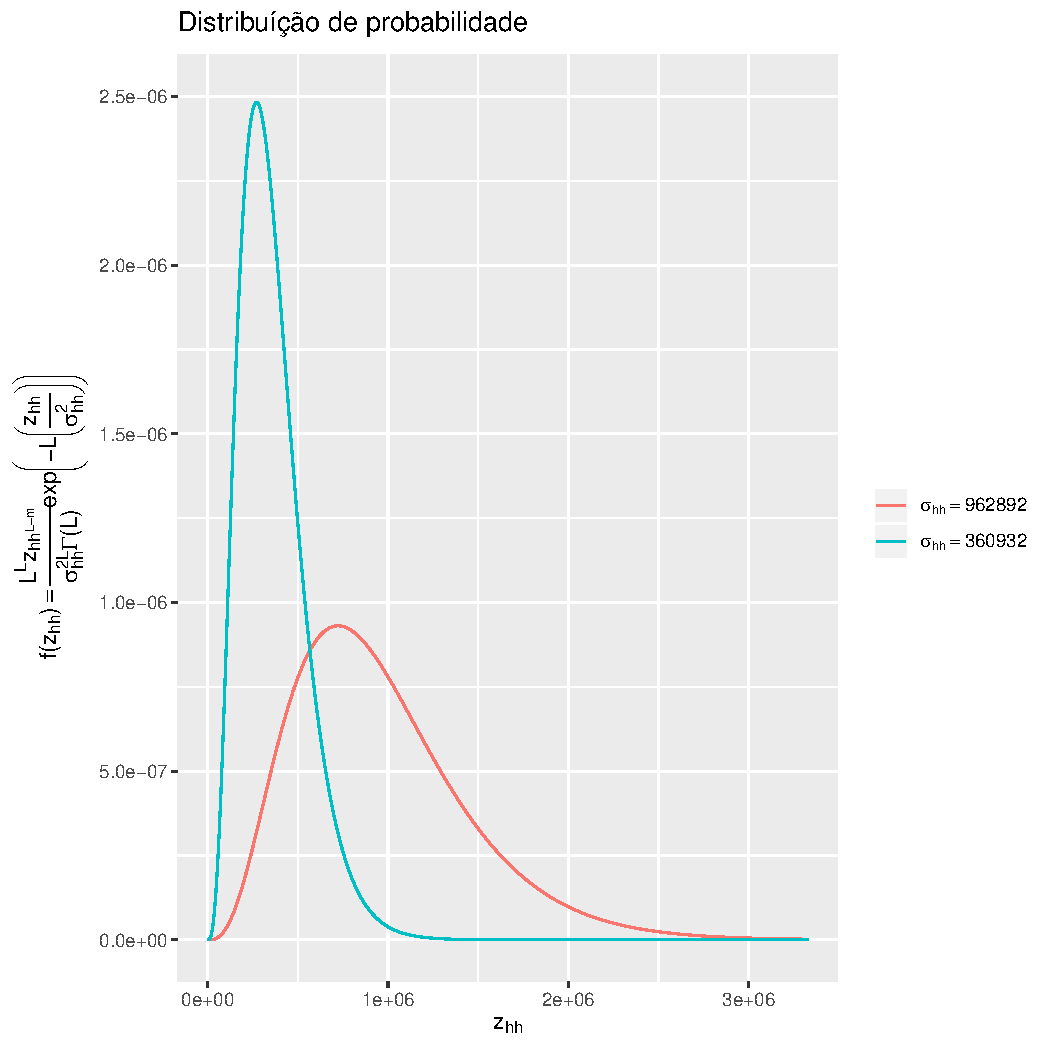
\includegraphics[scale = 0.4]{grafico_pdf_nhfc_2014_sigma_hh.pdf}
	\caption{Funções de densidade para dados simulados.}
\end{figure}  
\end{frame}
\begin{frame}{Detecção de bordas em imagens PolSAR}
  \begin{alertblock}{Estimativa de máxima verossimilhança - \textbf{MLE}}
  \begin{itemize}
\item Função de verossimilhança
\begin{equation}
    L(\theta;\mathbf{X}) = \prod_{i=1}^{n}f(x_i;\theta), 
\end{equation}
\item Função de log-verossimilhança
\begin{equation}
	l(\theta;\mathbf{X})= \ln(L(\theta;\mathbf{X})) = \sum_{i=1}^{n}\ln(f(x_i;\theta)),
\end{equation}
\item 
\begin{equation}
    \widehat{\theta}= \text{arg}\,\max\limits_{\theta\in\Theta}L(\theta;\mathbf{X}),
\end{equation}
\item
\begin{equation}
    \widehat{\theta}= \text{arg}\,\max\limits_{\theta\in\Theta}l(\theta;\mathbf{X}).
\end{equation}
\end{itemize}
\end{alertblock}
\end{frame}

\begin{frame}{Detecção de bordas em imagens PolSAR}
\alert{Estimativa de máxima verossimilhança, \cite{nhfc,gamf,gmbf} }
\begin{equation}
	L(j)=\prod_{k=1}^{j}f_{\mathbf{Z}}(\mathbf{Z}_{k}^{'};\Sigma_{A},L) \prod_{k=j+1}^{N}f_{\mathbf{Z}}(\mathbf{Z}_{k}^{'};\Sigma_{B},L), 
\end{equation}

\begin{equation}
	l(j)=\ln L(j)=\sum_{k=1}^{j}\ln f_{\mathbf{Z}}(\mathbf{Z}_{k}^{'};\Sigma_{A},L)+ \sum_{k=j+1}^{N}\ln f_{\mathbf{Z}}(\mathbf{Z}_{k}^{'};\Sigma_{B},L),
\end{equation}
\begin{equation*}
\begin{array}{rcl}
l(j)&=&N\left[mL\ln{\left(L\right)}-\ln{\left(\Gamma_m(L)\right)}\right]-L\left[j\ln{\left(|\Sigma_{A}|\right)} +(N-j)\ln{\left(|\Sigma_{B}|\right)}\right]\\
	&+&(L-m)\sum_{k=1}^{N}\ln{\left(|\mathbf{Z}_{k}^{'}|\right)}\\
        &-& L\left[\sum_{k=1}^{j}tr(\Sigma_{A}^{-1}\mathbf{Z}_{k}^{'})+ \sum_{k=j+1}^{N}tr(\Sigma_{B}^{-1}\mathbf{Z}_{k}^{'})\right]. 
\end{array}
\end{equation*}

\end{frame}
\begin{frame}{Detecção de bordas em imagens PolSAR}
\begin{alertblock}{Estimativa de máxima verossimilhança - \textbf{MLE}}
  \begin{itemize} \item
\begin{equation}
\widehat{\Sigma_{I}}(j) = \left\{
\begin{array}{lc}
	j^{-1}\sum_{k=1}^{j}\mathbf{Z}_{k}  & \mbox{se}\quad I=A,  \\
        (N-j)^{-1}\sum_{k=j+1}^{N}\mathbf{Z}_{k} & \mbox{se}\quad I=B, \\
\end{array}
\right.
\end{equation}
\item
\begin{equation}
\begin{array}{rcl}
	l(j)&=&N\left[-mL(1-\ln{\left(L\right)})-\ln{\left(\Gamma_m(L)\right)}\right]-L\left[j\ln{\left(|\widehat{\Sigma}_{A}(j)|\right)}\right. \\	
	&+&\left.(N-j)\ln{\left(|\widehat{\Sigma}_{B}(j)|\right)}\right] \\
	&+&(L-m)\sum_{k=1}^{N}\ln{\left(|\mathbf{Z}_{k}^{'}|\right)}, \\
\end{array}
\end{equation}
\item
\begin{equation}
	l(j)=-L\left[j\ln{\left(|\widehat{\Sigma}_{A}(j)|\right)}+(N-j)\ln{\left(|\widehat{\Sigma}_{B}(j)|\right)}\right],
\end{equation}
\item
\begin{equation}
	\widehat{\jmath}_{ML}=\text{arg}\max\limits_{j}l(j).  
\end{equation}
\end{itemize}
\end{alertblock}
\end{frame}
\begin{frame}{Detecção de bordas em imagens PolSAR}
  \begin{figure}[hbt]
\minipage{0.30\textwidth}
  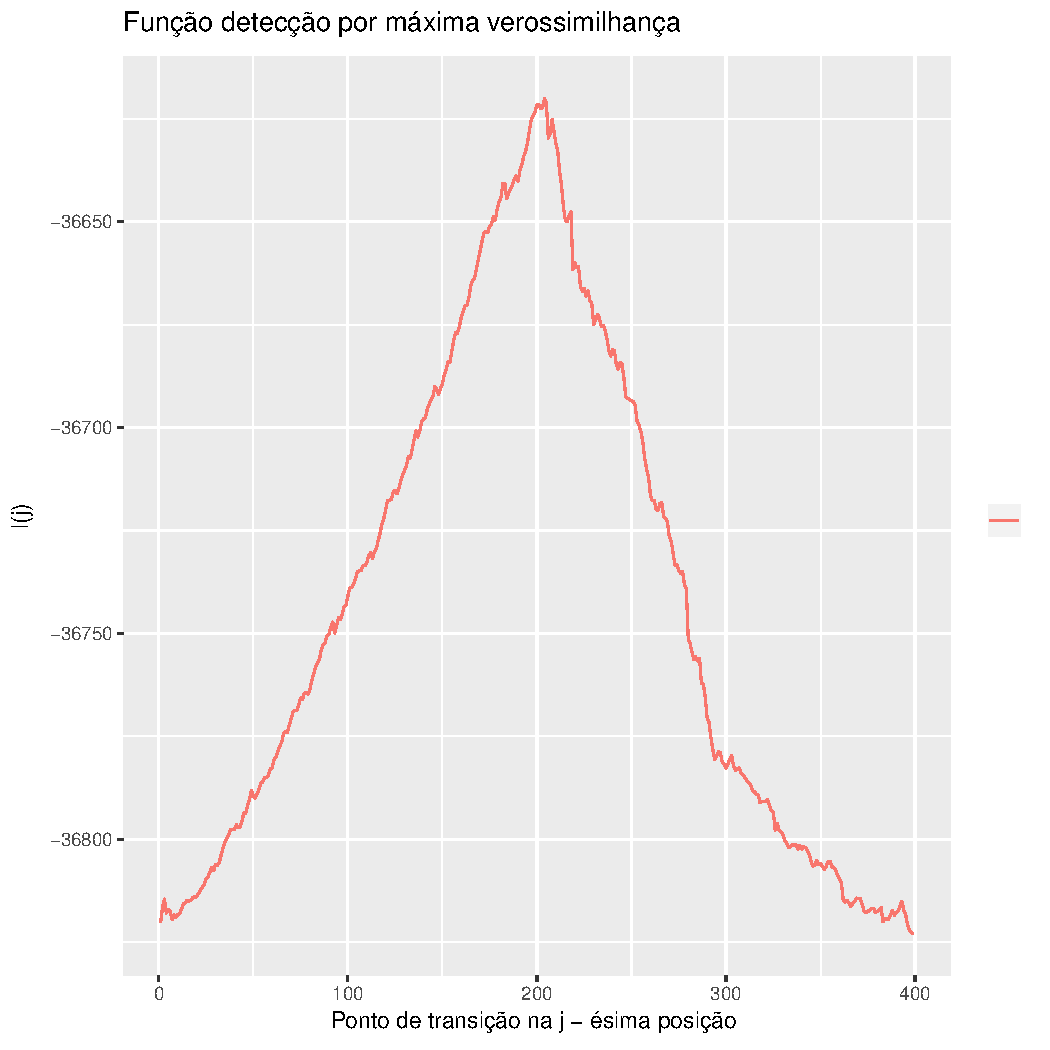
\includegraphics[width=\linewidth]{grafico_l_nhfc_2014_sigmahh.pdf}
	\caption{Função $l(j)$ para o canal $I_{HH}$.}
\endminipage\hfill
\minipage{0.30\textwidth}
  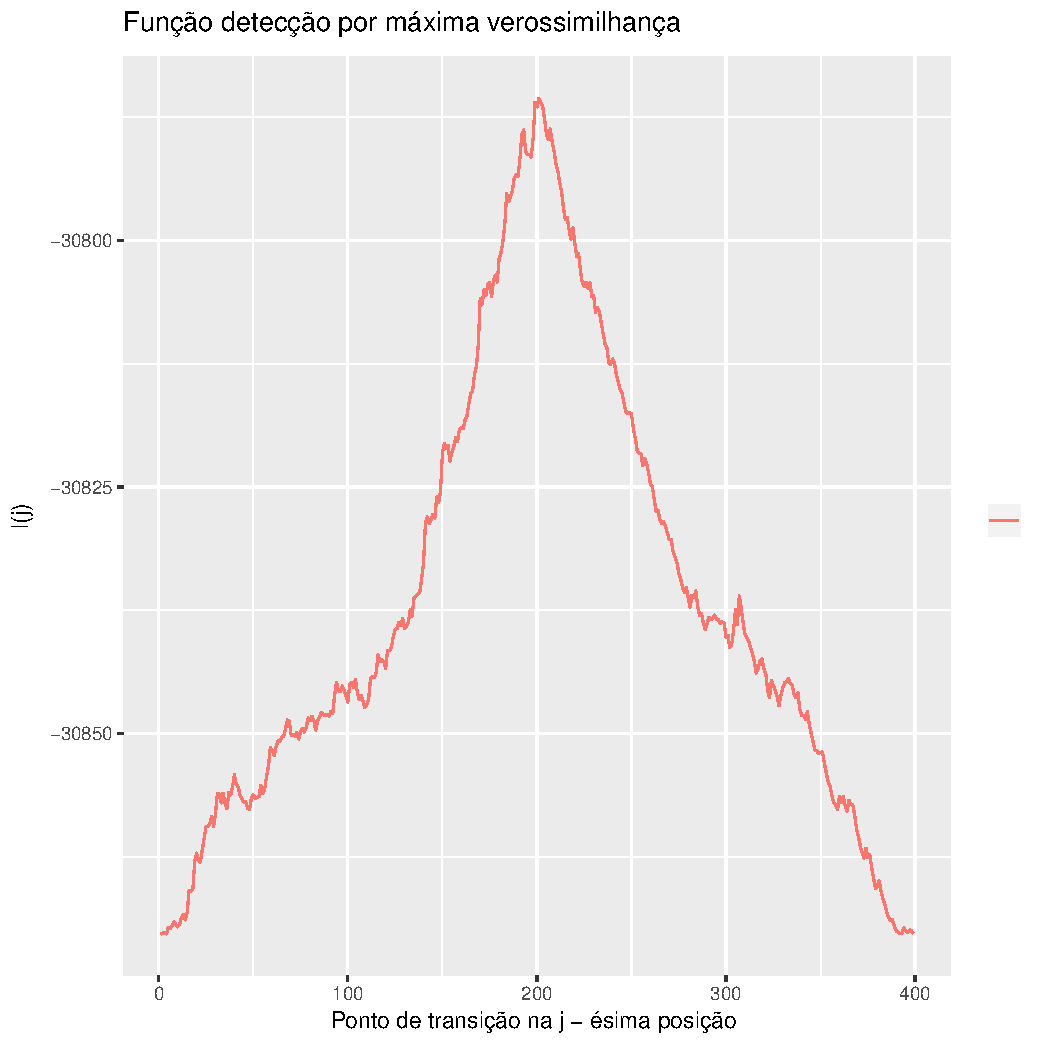
\includegraphics[width=\linewidth]{grafico_l_nhfc_2014_sigmahv.pdf}
	\caption{Função $l(j)$ para o canal $I_{HV}$.}
\endminipage\hfill
\minipage{0.30\textwidth}
  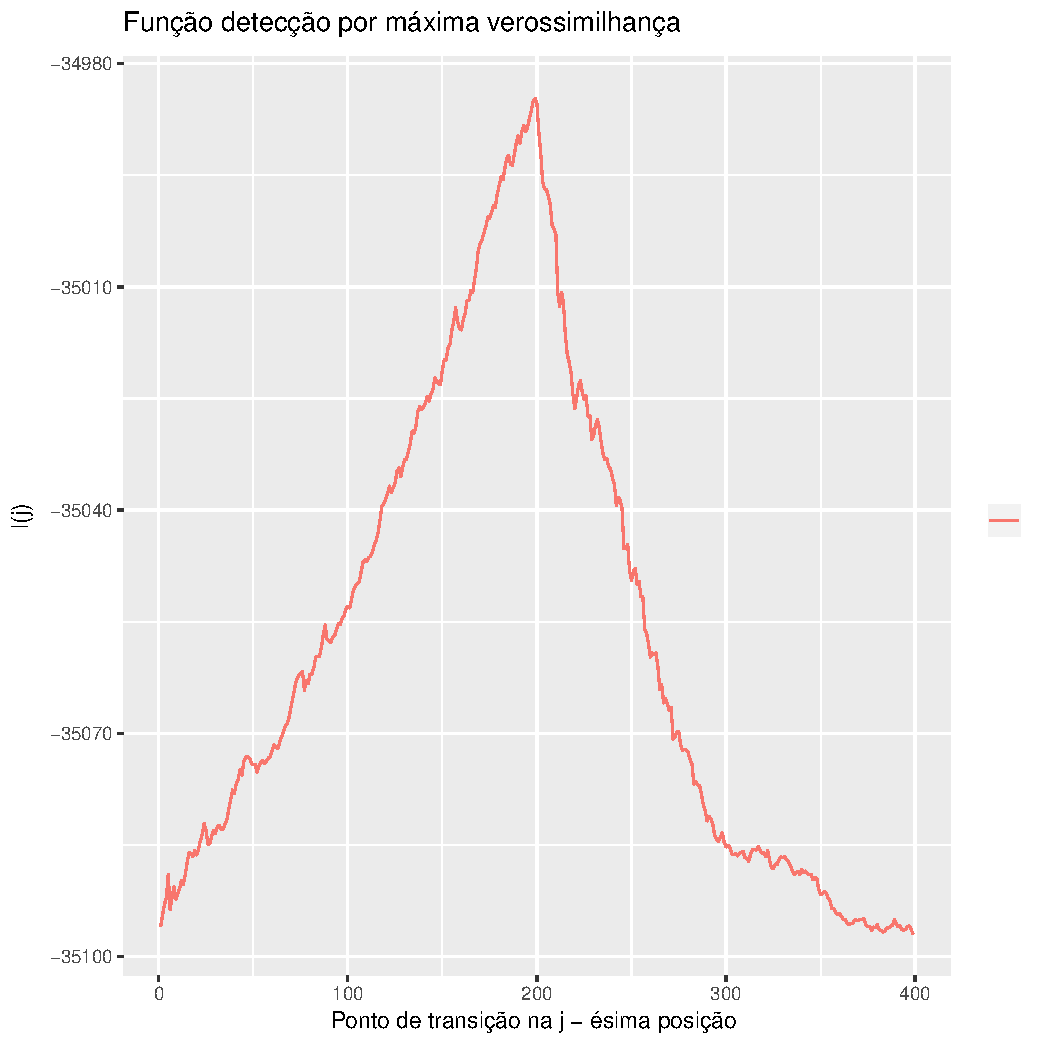
\includegraphics[width=\linewidth]{grafico_l_nhfc_2014_sigmavv.pdf}
	\caption{Função $l(j)$ para o canal $I_{VV}$.}
\endminipage\hfill
\end{figure}
\end{frame}
\begin{frame}{Detecção de bordas em imagens PolSAR}
\begin{alertblock}{Metodologia de detecção de bordas (para cada canal)}
\begin{enumerate}
    \item Definir uma região de interesse (ROI) de maneira automática, semiautomática ou manual;
	\item calcular o centróide da (ROI); 
	\item construir raios partindo do centróide e indo para fora da área de interesse (Bresenham's line algorithm);
	\item coletar dados em uma vizinhança em torno dos raios, construir $l(j)$ ;
	\item detectar pontos na faixa de dados, os quais fornecem evidências de mudanças de propriedades estatísticas, para isso, usamos o método GenSA.
\end{enumerate}
\end{alertblock}
\end{frame}
\begin{frame}{Detecção de bordas em imagens PolSAR}
\begin{alertblock}{Metodologia de detecção de bordas com fusão de evidências}
\begin{enumerate}
    \item Aplicar o método de fusão de evidências;
	\item definir o contorno usando um método de interpolação entre os pontos provenientes da fusão de evidências, por exemplo, as B-Splines, ou o método dos quadrados mínimos \textbf{MMQ}.
\end{enumerate}
\end{alertblock}
\end{frame}


\section{Resultados numéricos}
\begin{frame}{Resultados numéricos}
\begin{alertblock}{Otimização}
  \begin{itemize}
\item MaxLik
  	\begin{itemize}
	\item Métodos de otimização - Gradiente - Hessiano;
	\item NR   - Newton-Raphson (diferenças finitas ou analítico); 
	\item BHHH - Berndt-Hall-Hall-Hausman (diferenças finitas ou analítico);
	\item BFGS - Broyden-Fletcher-Goldfarb-Shanno (diferenças finitas ou analítico);
	\item NM   - Nelder-Mead  (não calcula);
        \item SANN - simulated annealing (não calcula).
	\end{itemize}
\item GenSA;
\item Generalized Simulated Annealing.
\end{itemize}
\end{alertblock}
\end{frame}

\begin{frame}{Resultados numéricos}
\alert{GenSA aplicado em $l(j)$ nos respectivos canais.}
\begin{figure}[hbt]
\minipage{0.3\textwidth}
  \fbox{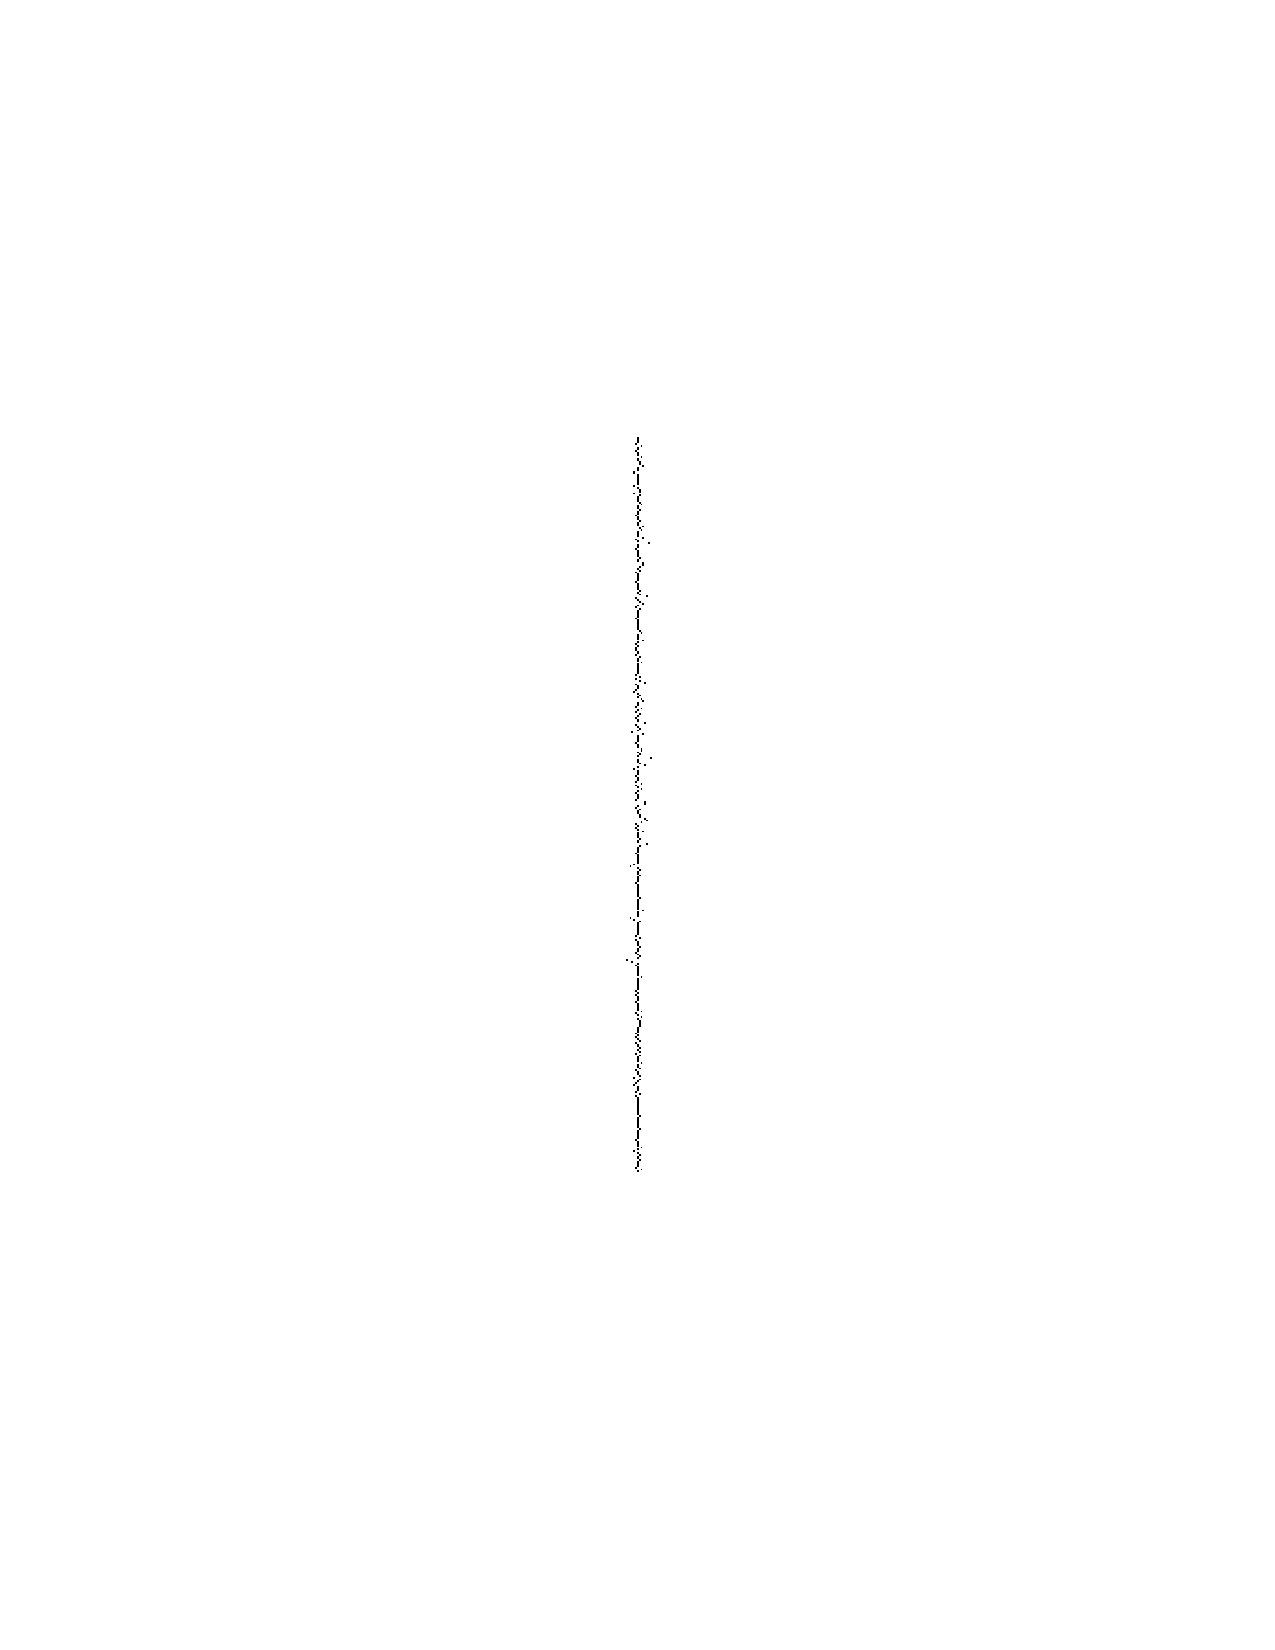
\includegraphics[width=\linewidth]{ev_hh_nhfc_2014.pdf}}
\caption{Evidências de bordas no canal $I_{HH}$.}
\endminipage\hfill
\minipage{0.3\textwidth}
\fbox{ 
\includegraphics[width=\linewidth]{ev_hv_nhfc_2014.pdf}}
\caption{Evidências de bordas no canal $I_{HV}$.}
\endminipage\hfill
\minipage{0.3\textwidth}
\fbox{ 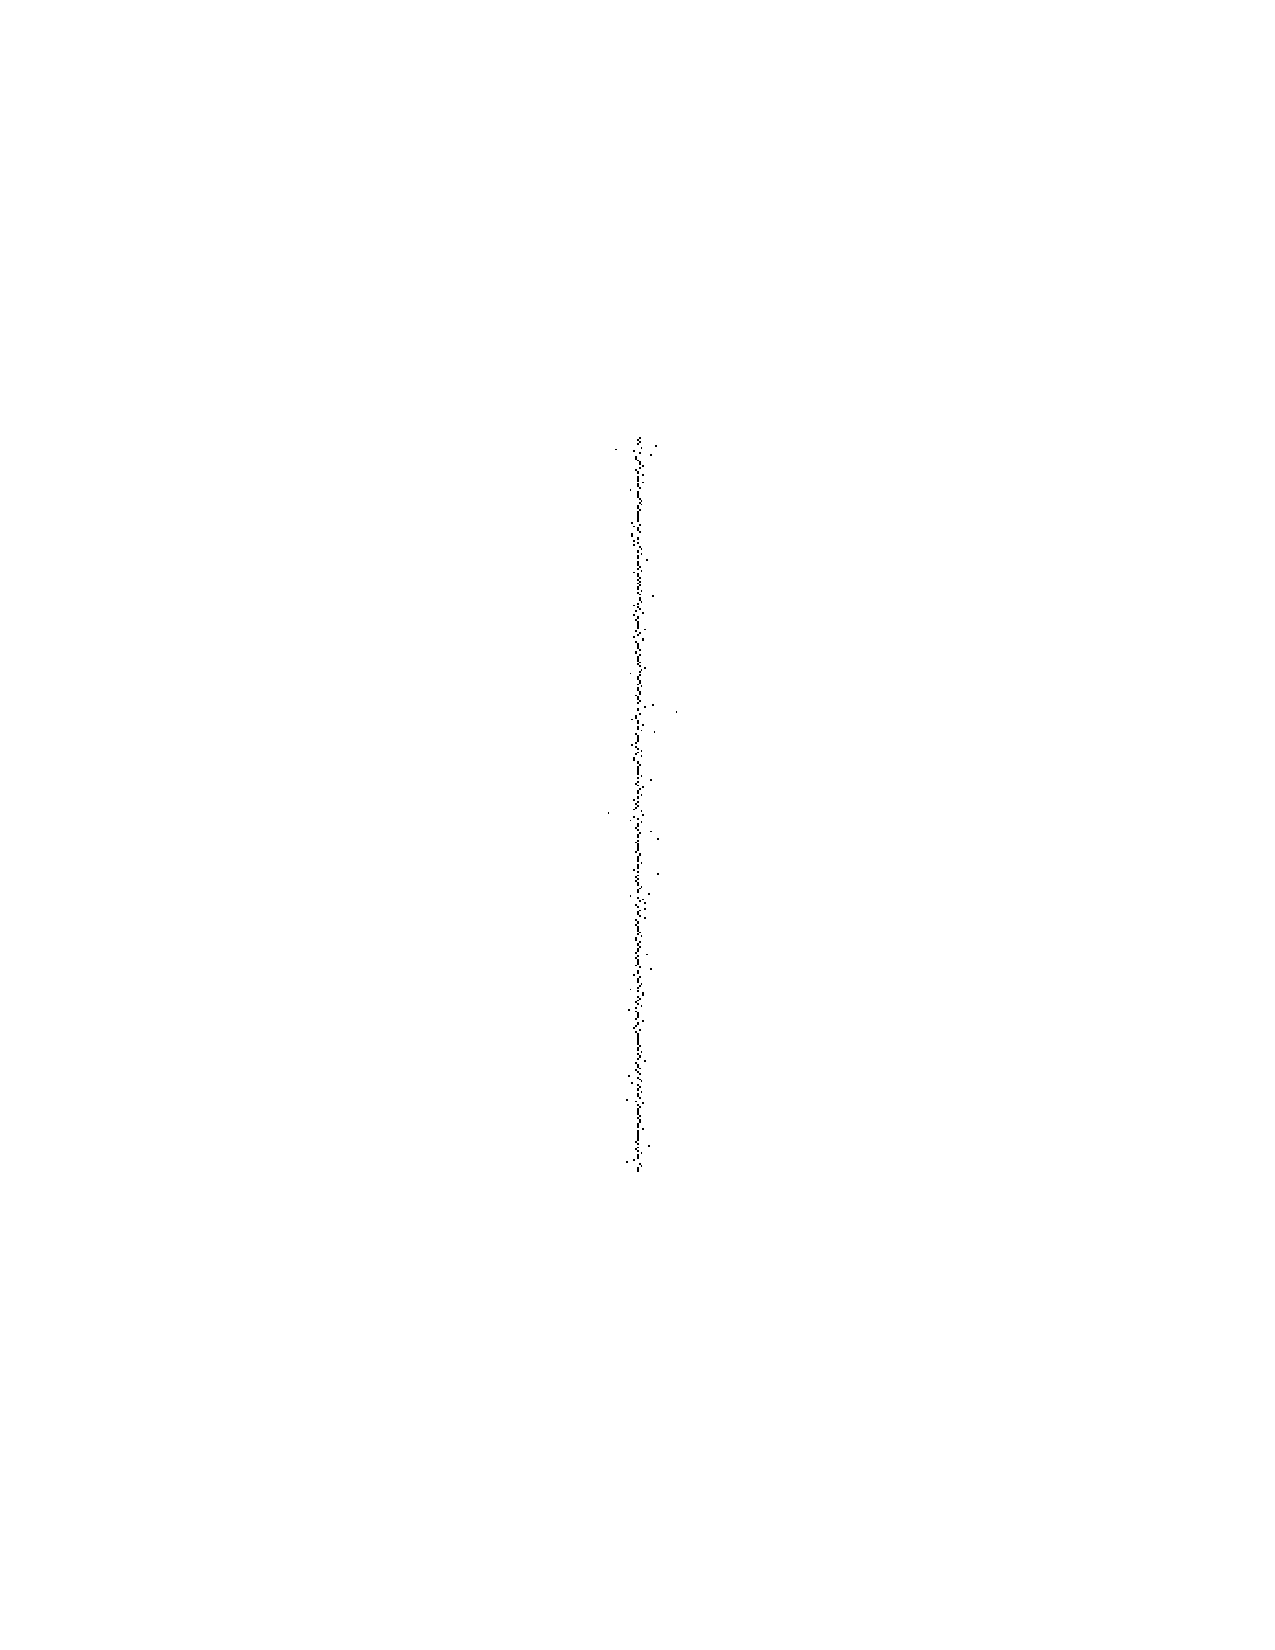
\includegraphics[width=\linewidth]{ev_vv_nhfc_2014.pdf}}
\caption{Evidências de bordas no canal $I_{VV}$.}
\endminipage\hfill
\end{figure}
\end{frame}
\begin{frame}{Resultado numéricos}
\alert{Fusão de evidências de bordas, \cite{mit}}
  \begin{equation}
\begin{array}{lll}
	F_{m}^{ev} &=&\frac{1}{K}\displaystyle{\sum_{k=1}^{K}ev_k}. 
\end{array}
\end{equation}
	\begin{itemize}
	\item $m$ - dimensão do vetor de evidências de bordas;
        \item $K$ - Número de canais.
	\end{itemize}
\end{frame}

\begin{frame}{Resultados numéricos}
\alert{Fusão de evidências e Quadrados mínimos}
\begin{figure}[hbt]
\minipage{0.40\textwidth}
	\fbox{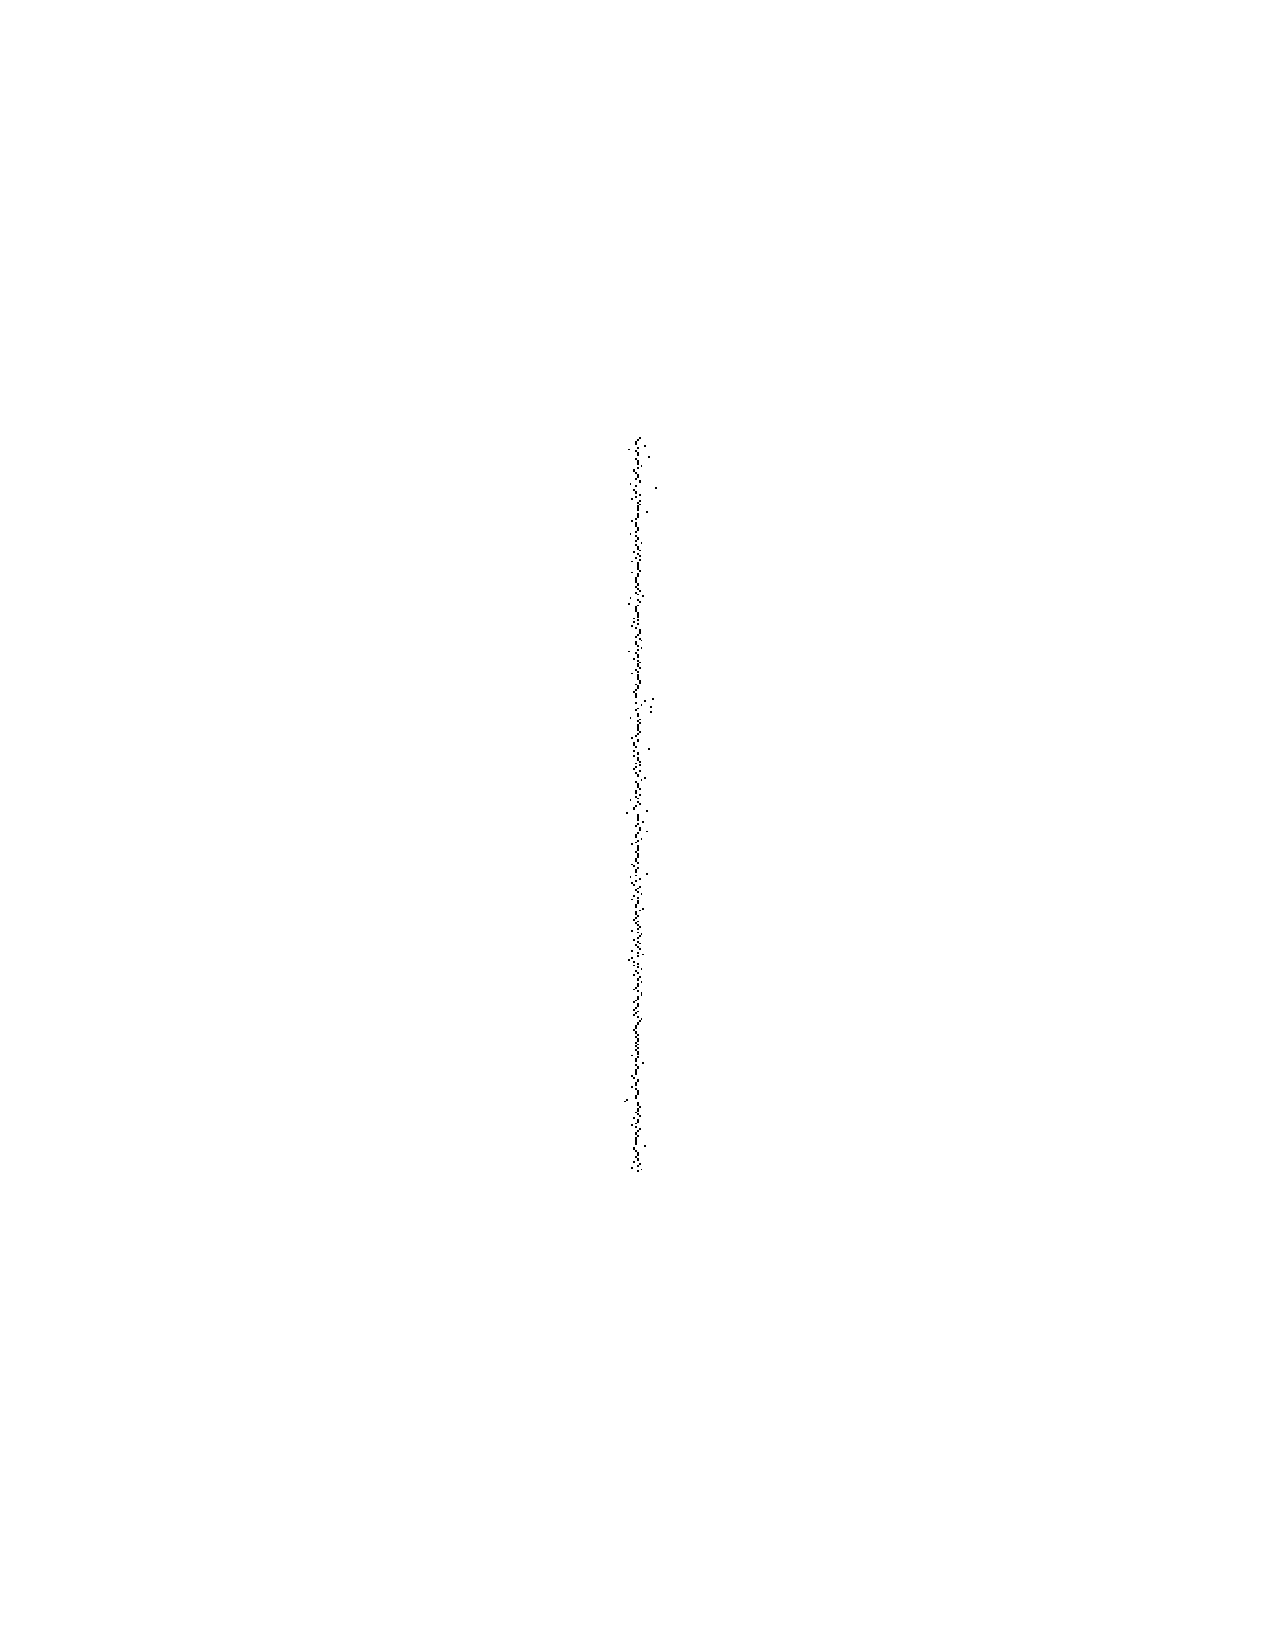
\includegraphics[width=\linewidth]{fusao_soma_ev_hh_hv_vv_nhfc.pdf}}
	\caption{Fusão de evidências para os canais $\left(I_{hh}, I_{hv}, I_{vv}\right)$.}
\endminipage\hfill
\minipage{0.40\textwidth}
\fbox{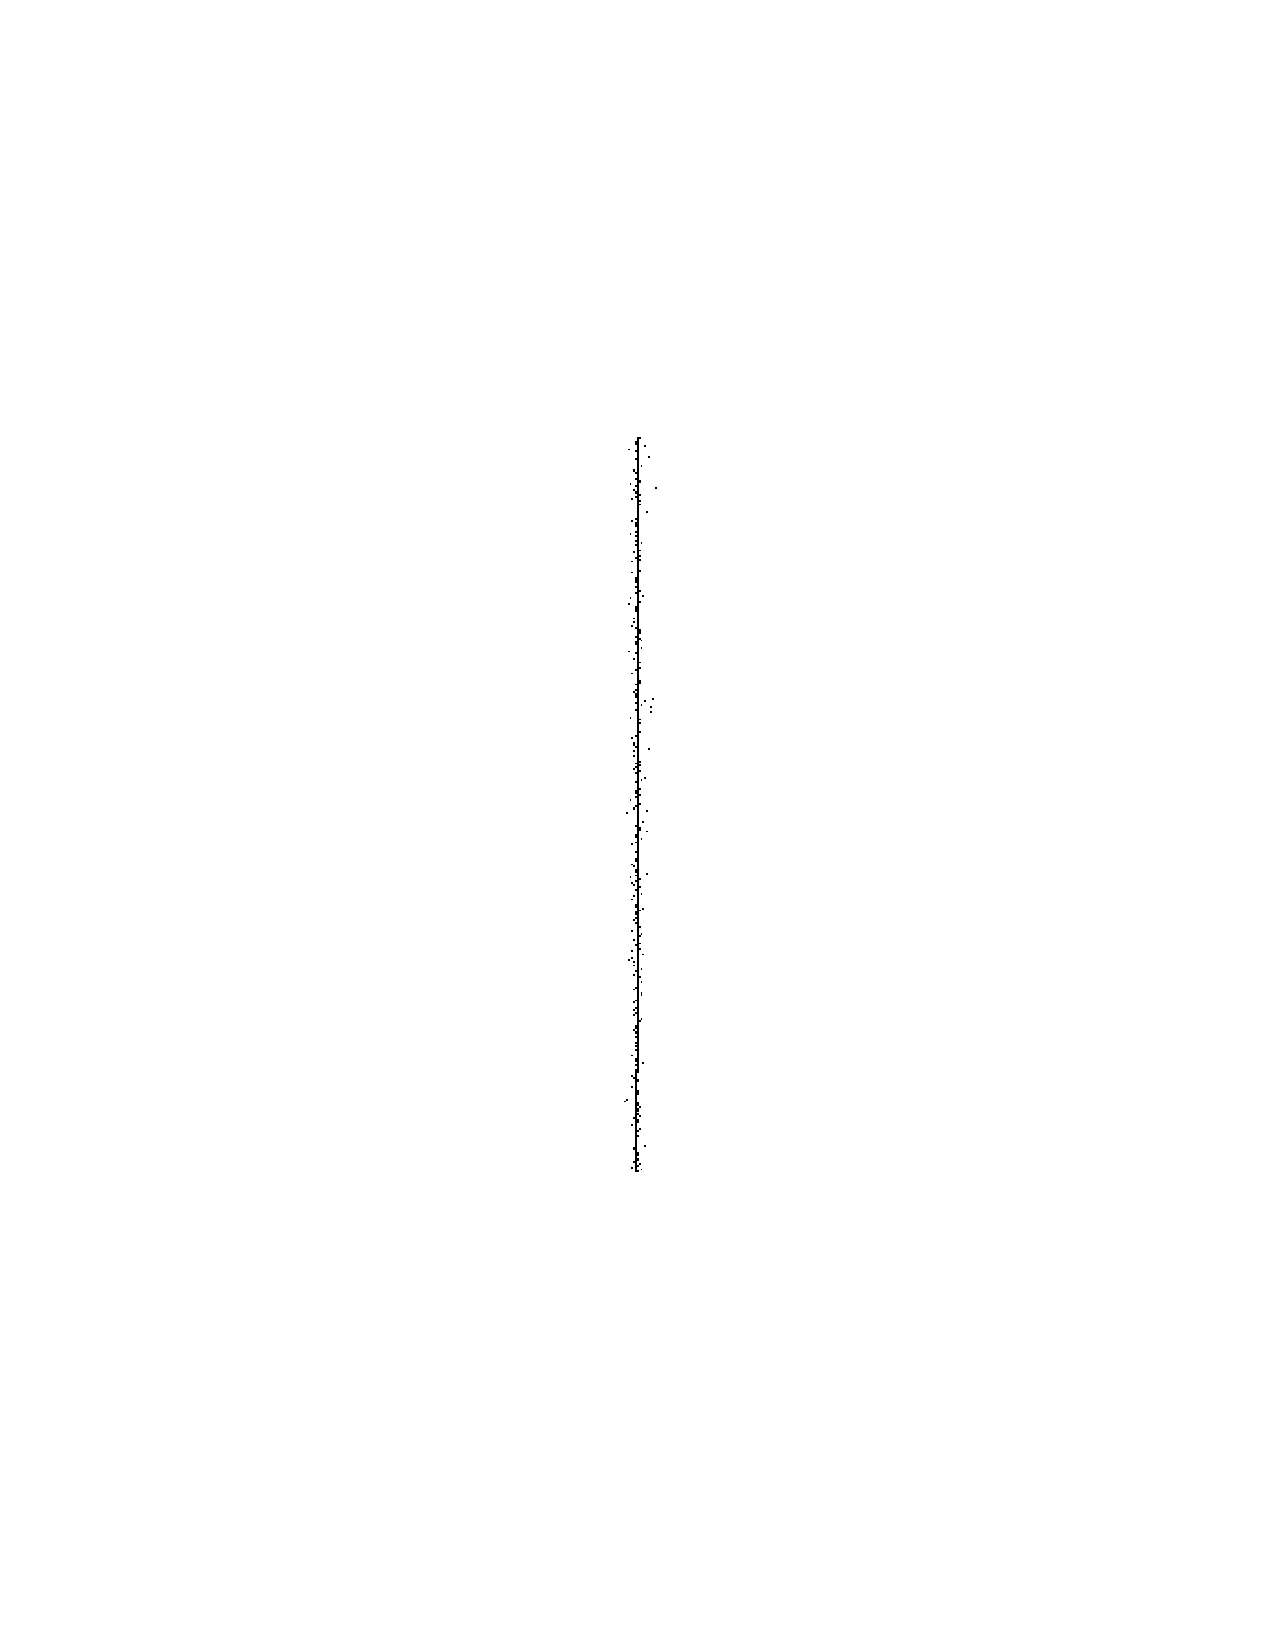
\includegraphics[width=\linewidth]{fusao_ls_nhfc.pdf}}	
\caption{Método dos quadrados mínimos.}
\endminipage\hfill
\end{figure}
\end{frame}
\begin{frame}{Resultados numéricos}
\begin{alertblock}{Probabilidade de detecção, \cite{gmbf}.}
\begin{enumerate}
    \item Foi replicado o método de detecção de bordas $r=400$ vezes e calculado o erro $E(r)=|b - pt(r)|$, onde $b=200$ e $pt(r)$ é o vetor com as $r$ replicações;
    \item vamos usar frequências relativas com objetivo de estimar a probabilidade de ter um erro menor que um certo número de pixeis;
    \item sendo $H(k)$ o número de replicações tal que o erro é menor que $k$ pixeis, então a probabilidade é $f(k)=\frac{H(k)}{400}$, com $k=1,\cdots,10$. 
\end{enumerate}
\end{alertblock}
\end{frame}
\begin{frame}{Resultados numéricos}
\begin{figure}[hbt]
\minipage{0.475\textwidth}
	\fbox{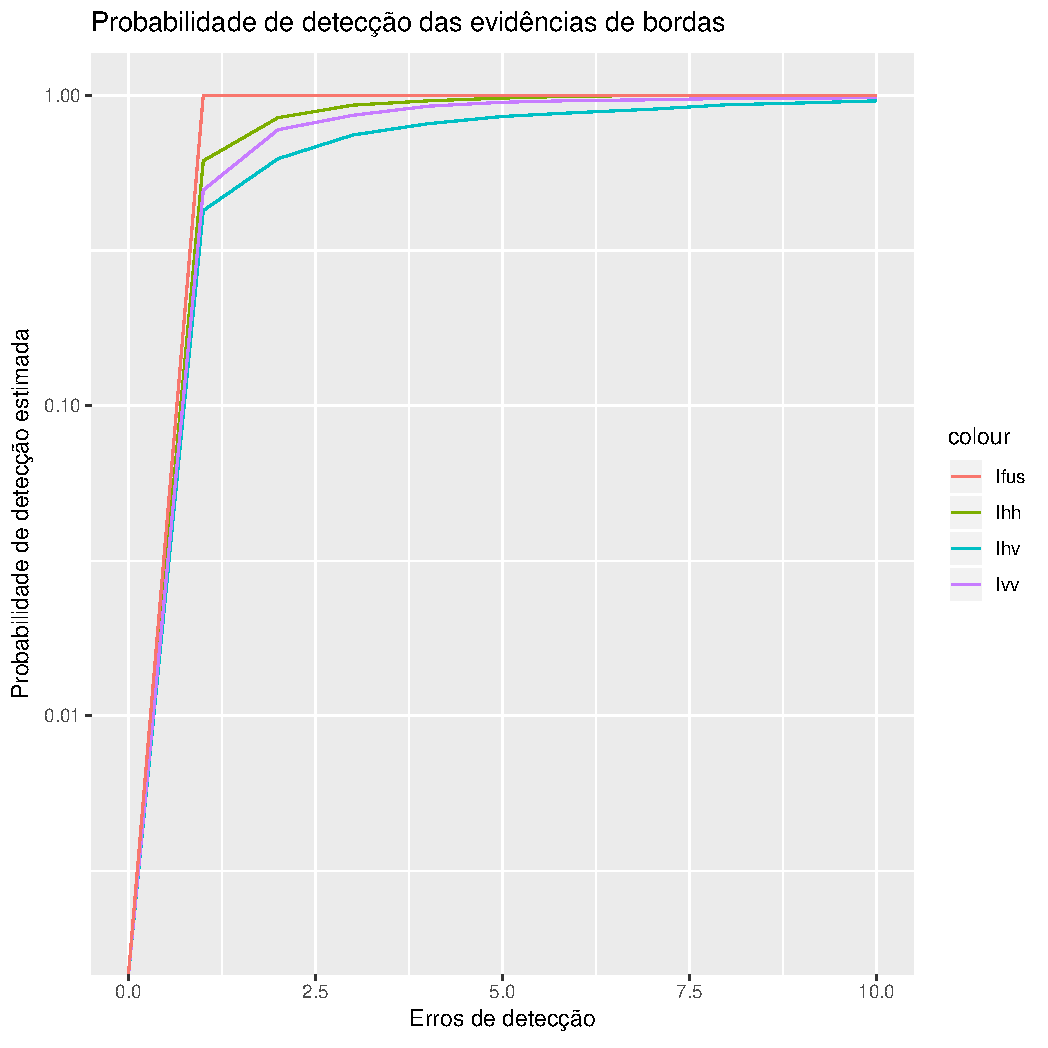
\includegraphics[width=\linewidth]{metricas_ihh_ivh_ivv_ils_nhfc.pdf}}
	\caption{Probabilidade de detecção de borda com fusão de evidências nos respectivos canais.}
\endminipage\hfill
\minipage{0.475\textwidth}
\fbox{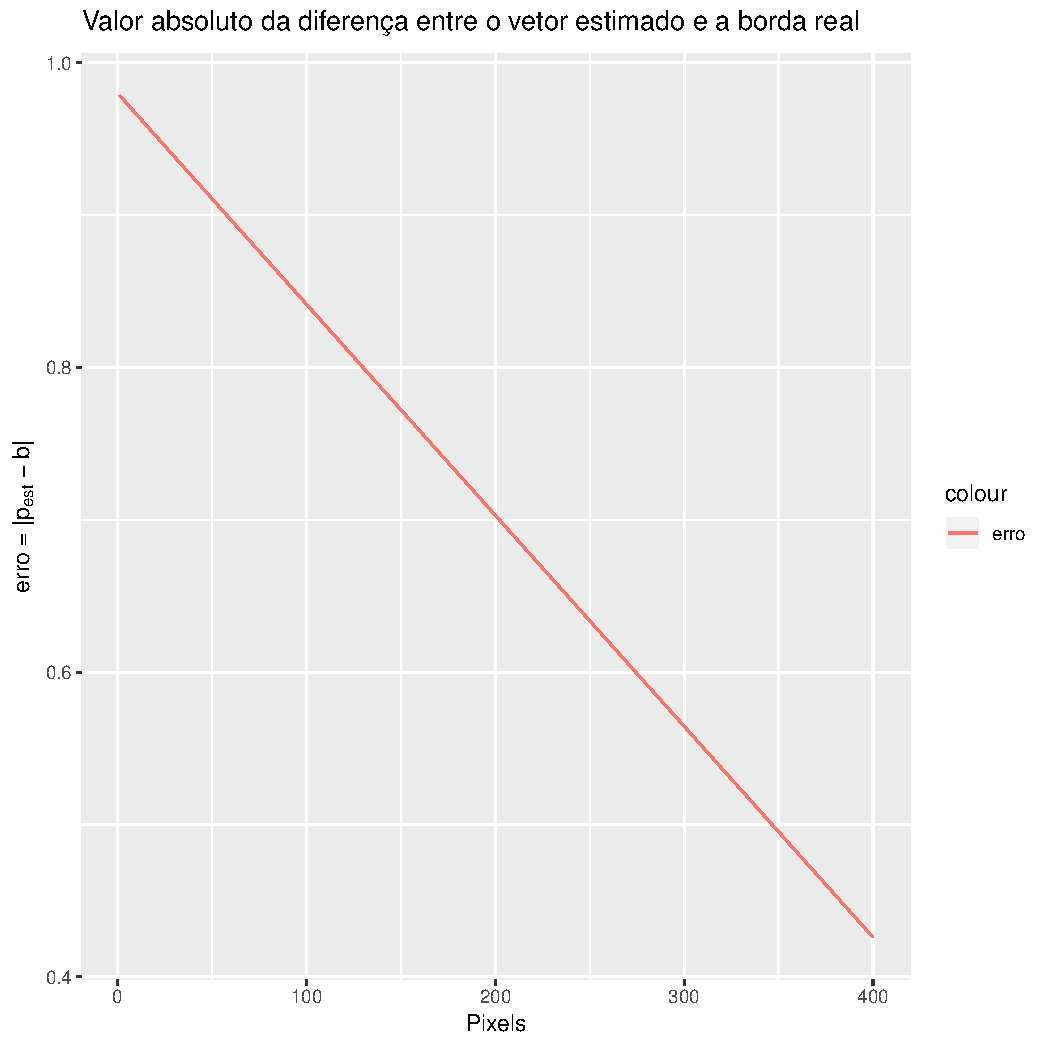
\includegraphics[width=\linewidth]{fusao_ls_erro_nhfc.pdf}}	
	\caption{Valor absoluto da diferença entre o vetor estimado da fusão de evidências e a borda real.}
\endminipage\hfill
\end{figure}
\end{frame}
\begin{frame}{Resultados numéricos}
\begin{figure}[hbt]
\minipage{0.45\textwidth}
	\fbox{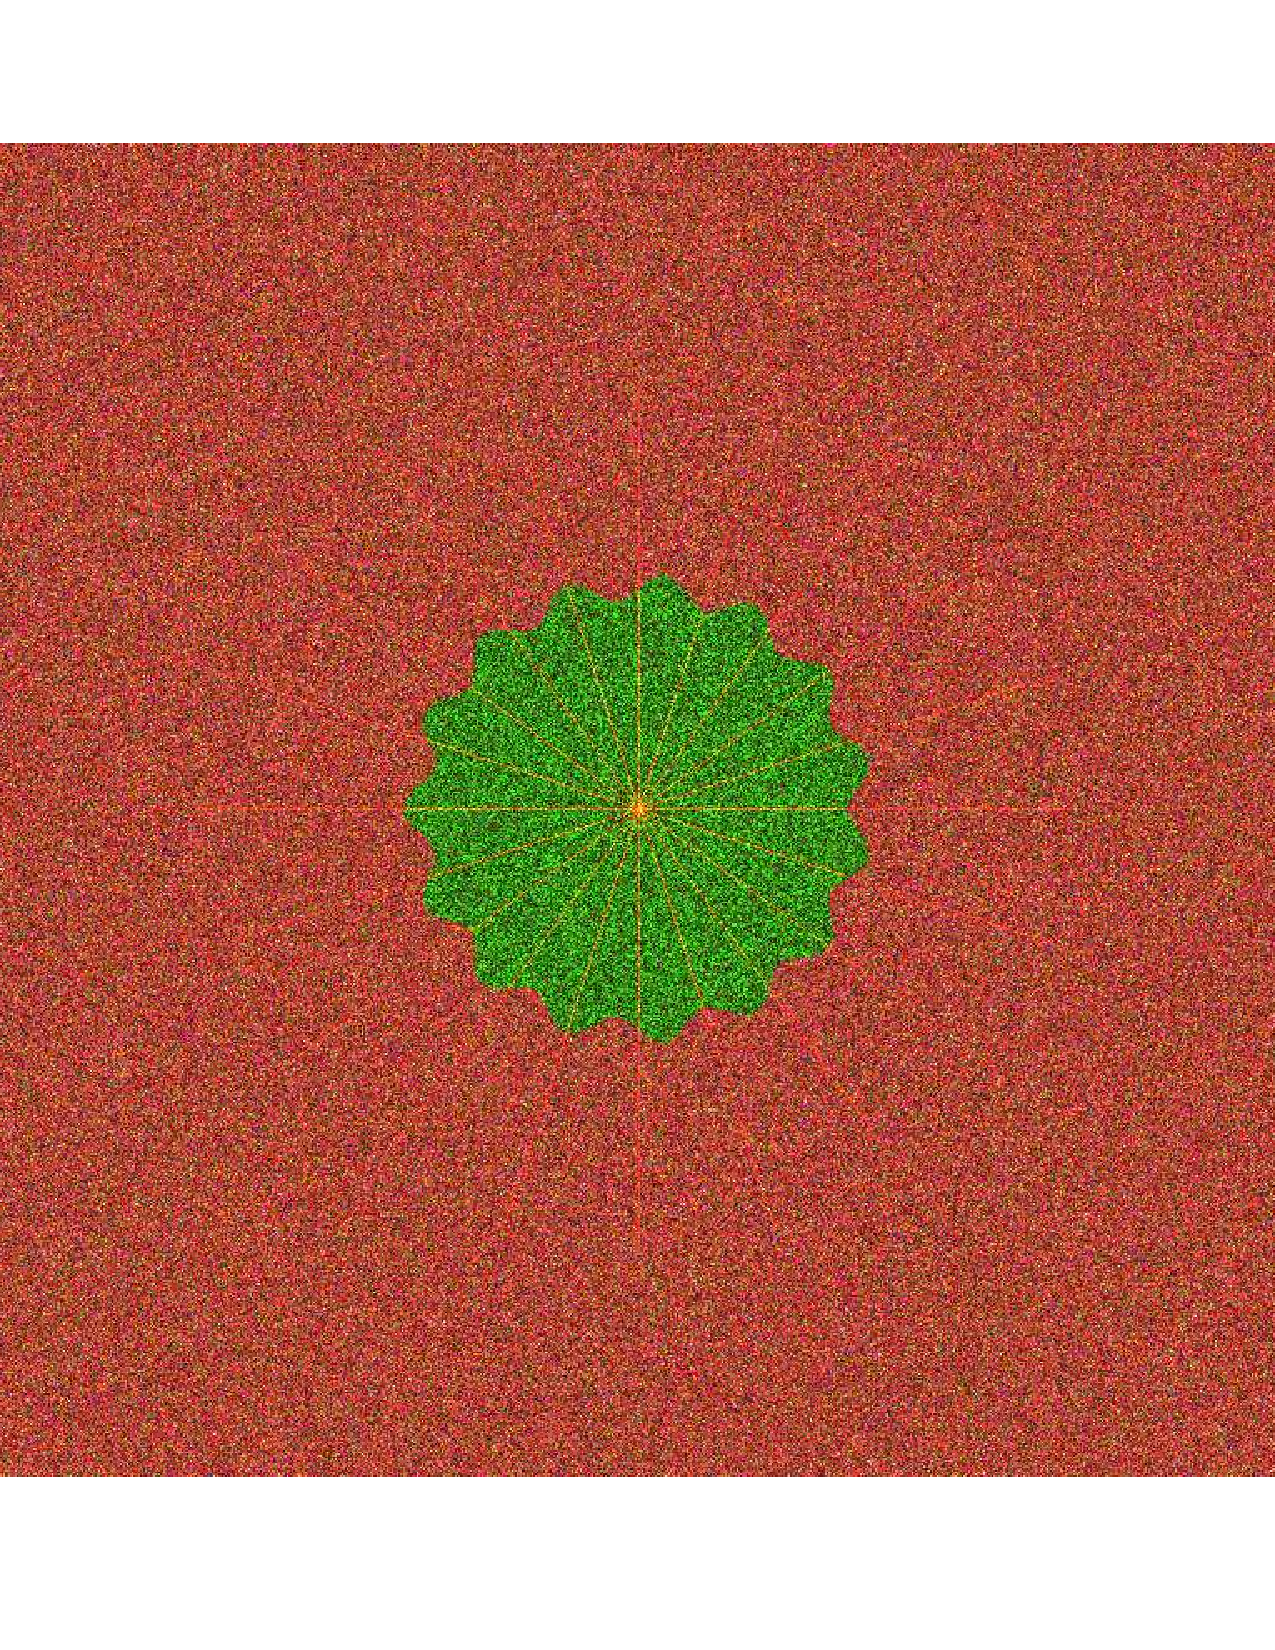
\includegraphics[width=\linewidth]{flor_15_133_8_pauli.pdf}}
	\caption{Imagem flor simulada com parâmetros $\beta = 15$, $\delta = 133$ e $\nu = 8$ .}
\endminipage\hfill
\minipage{0.45\textwidth}
\fbox{
\includegraphics[width=\linewidth]{flor_15_133_8_bin.pdf}}	
	\caption{Imagem flor simulada binária com $\beta = 15$, $\delta = 133$ e $\nu = 8$ .}
\endminipage
\end{figure}
\end{frame}

\begin{frame}{Resultados numéricos}
\begin{figure}[hbt]
\minipage{0.3\textwidth}
\fbox{  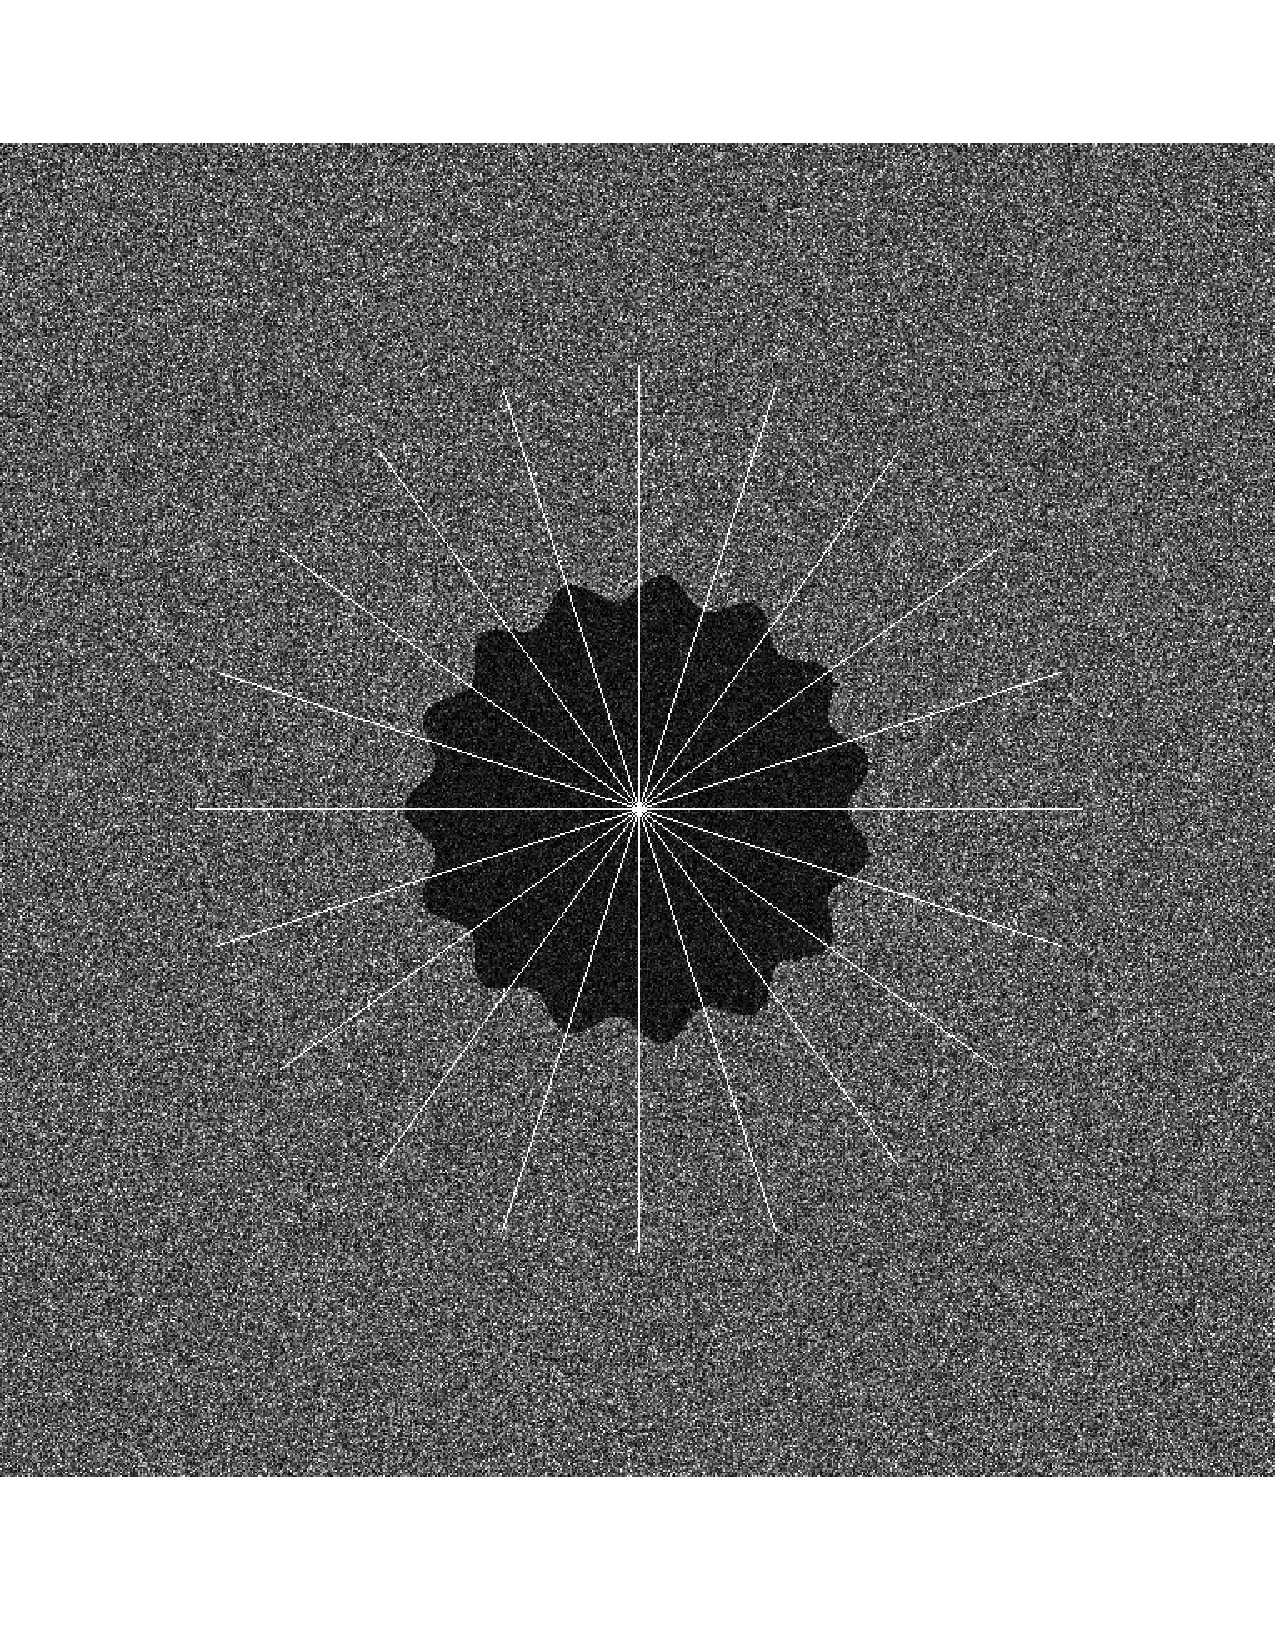
\includegraphics[width=\linewidth]{flor_15_133_8_hh.pdf}}
	\caption{Imagem flor simulada canal $I_{hh}$ com $\beta = 15$, $\delta = 133$ e $\nu = 8$ .}
\endminipage\hfill
\minipage{0.3\textwidth}
\fbox{ 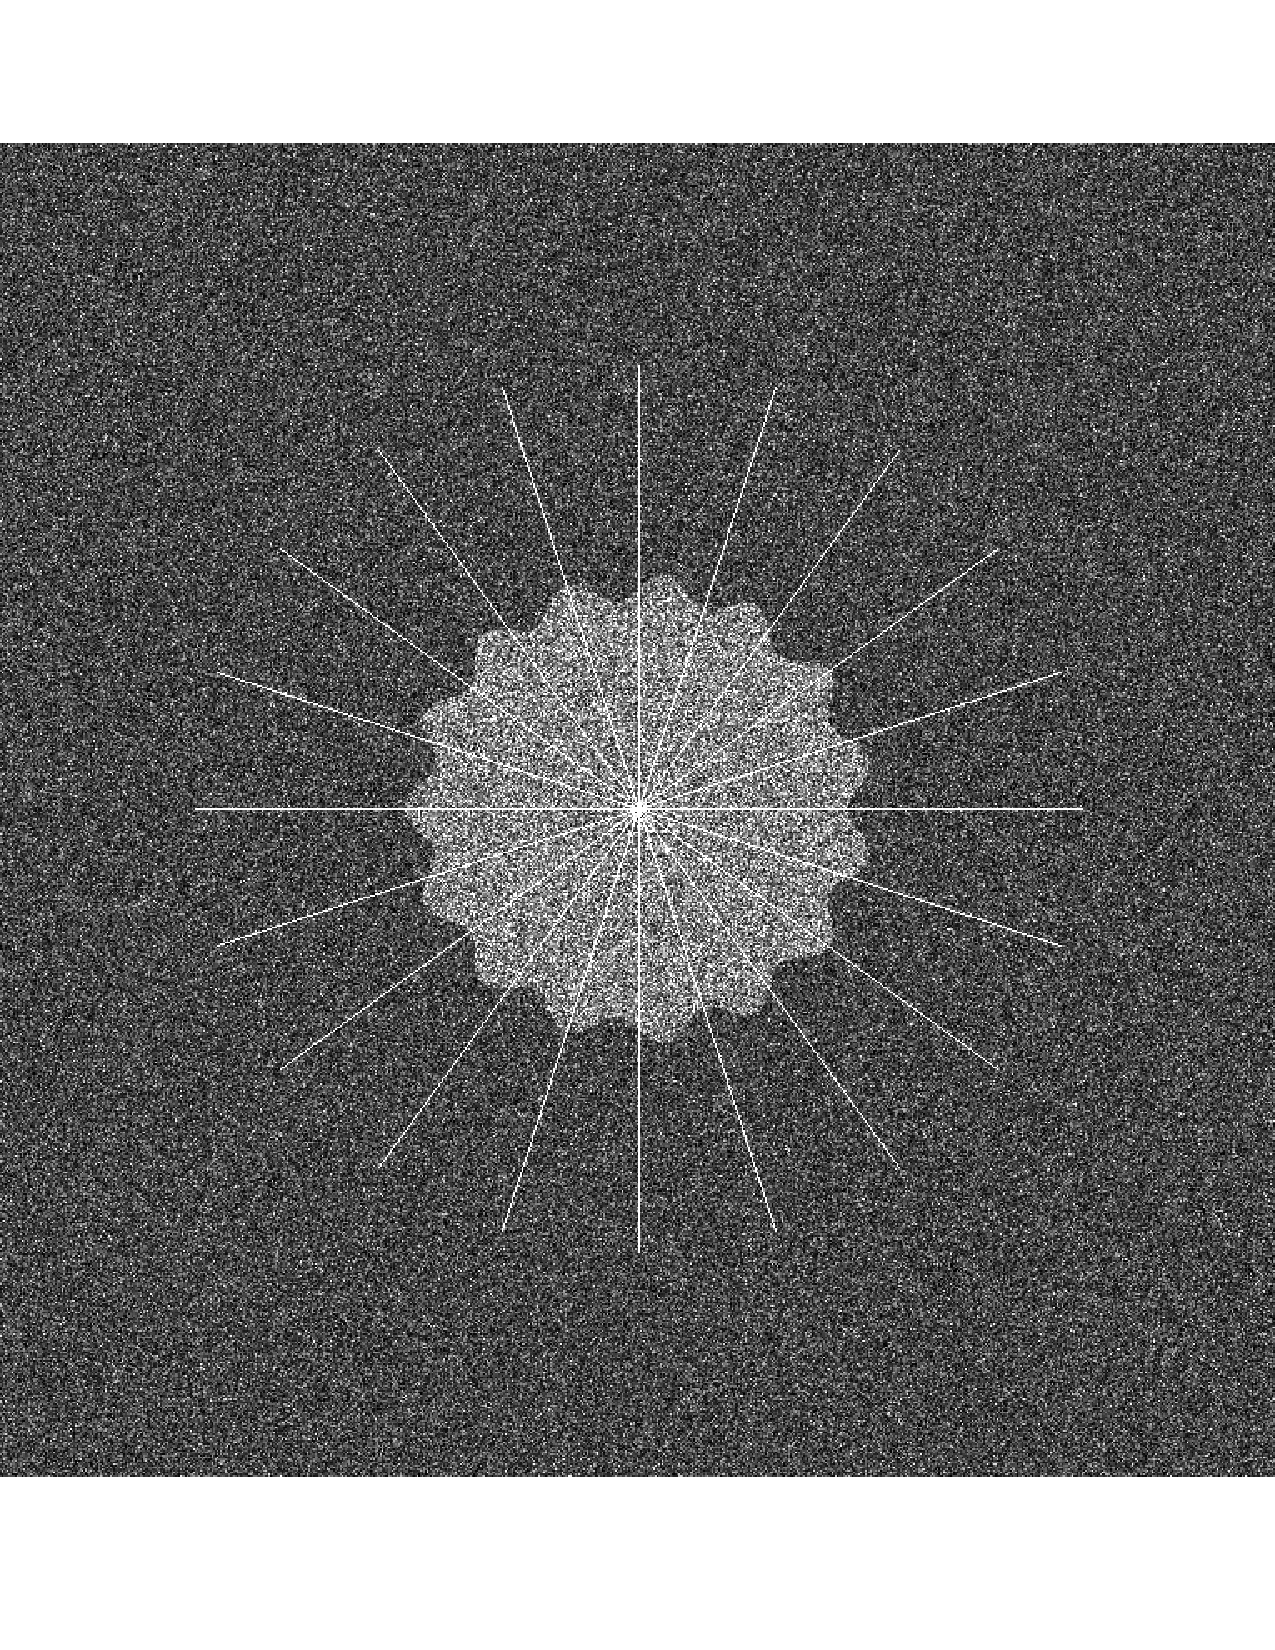
\includegraphics[width=\linewidth]{flor_15_133_8_hv.pdf}}
	\caption{Imagem flor simulada canal $I_{hv}$ com $\beta = 15$, $\delta = 133$ e $\nu = 8$ .}
\endminipage\hfill
\centering
\minipage{0.3\textwidth}
\fbox{ 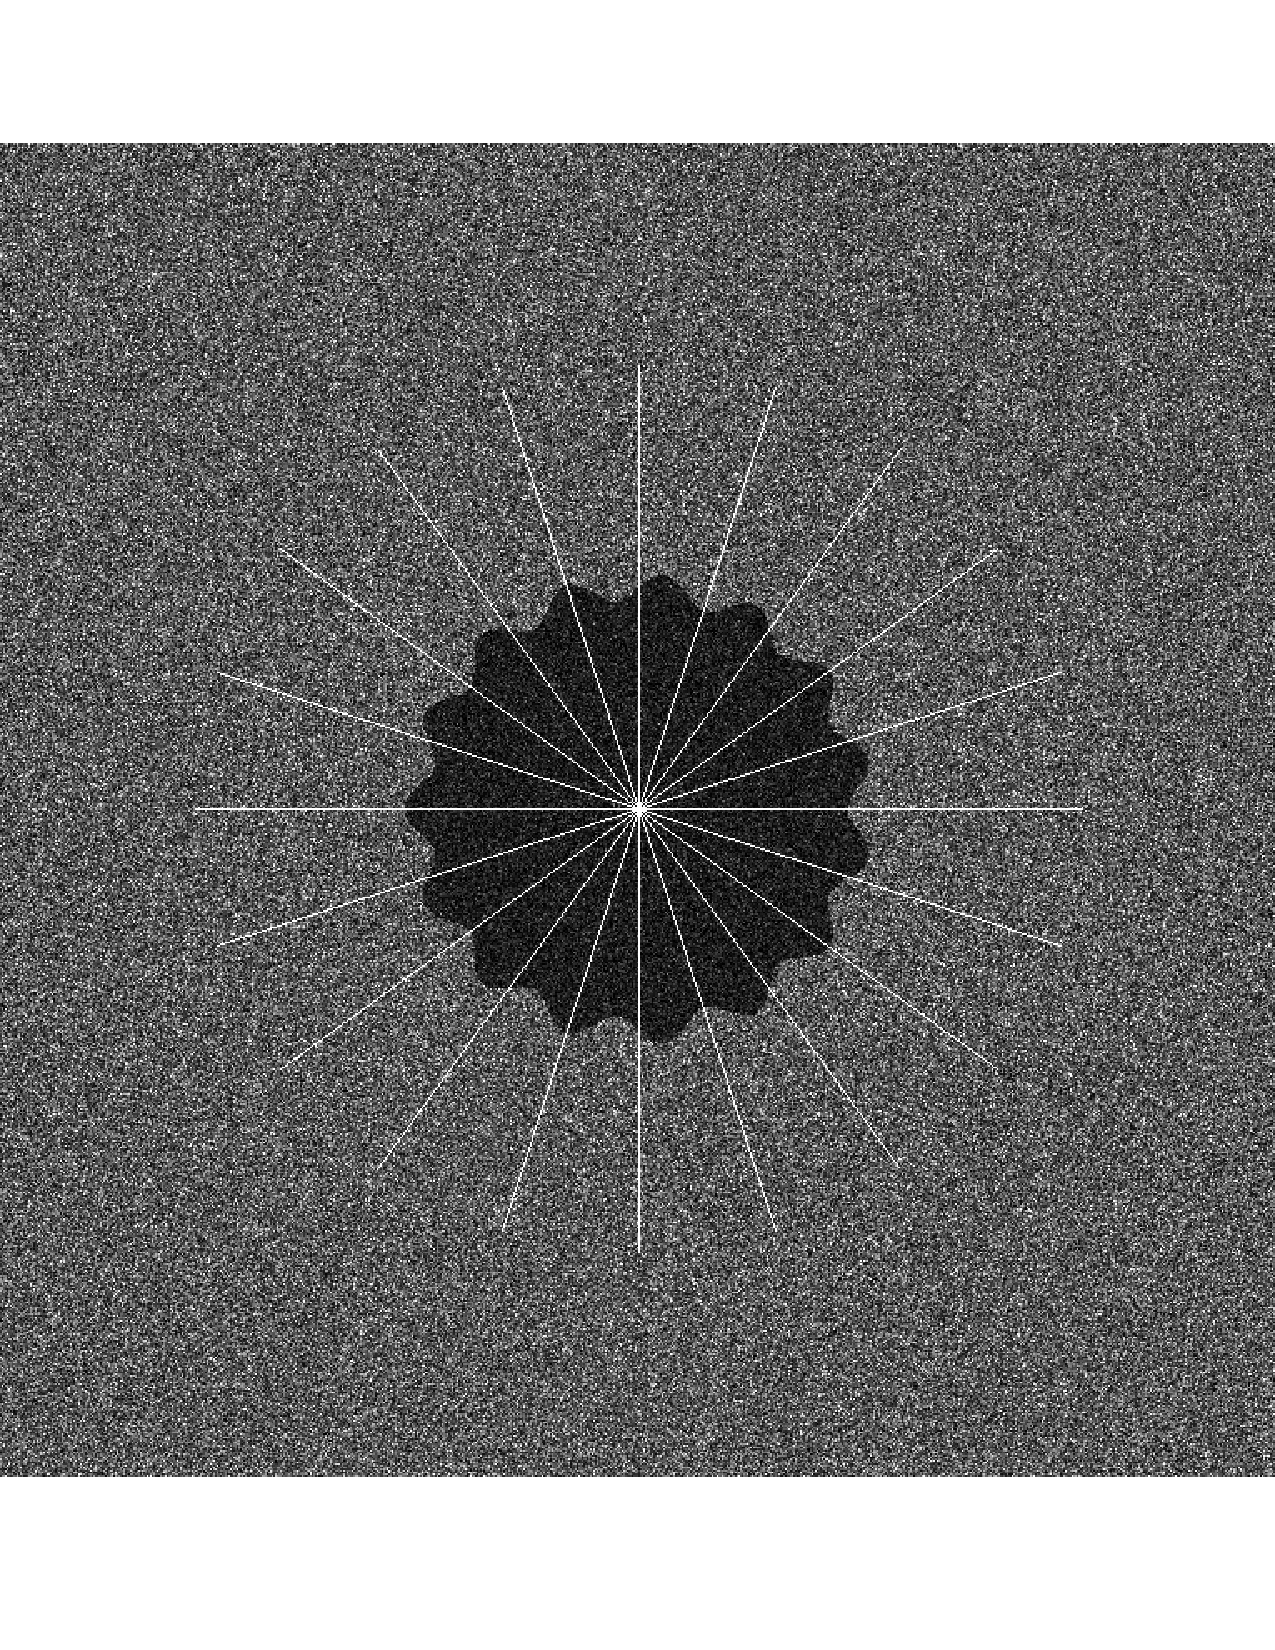
\includegraphics[width=\linewidth]{flor_15_133_8_vv.pdf}}
	\caption{Imagem flor simulada canal $I_{vv}$ com $\beta = 15$, $\delta = 133$ e $\nu = 8$ .}
\endminipage\hfill
\end{figure}
 
\end{frame}

\begin{frame}{Resultados numéricos}
\begin{figure}[hbt]
	\fbox{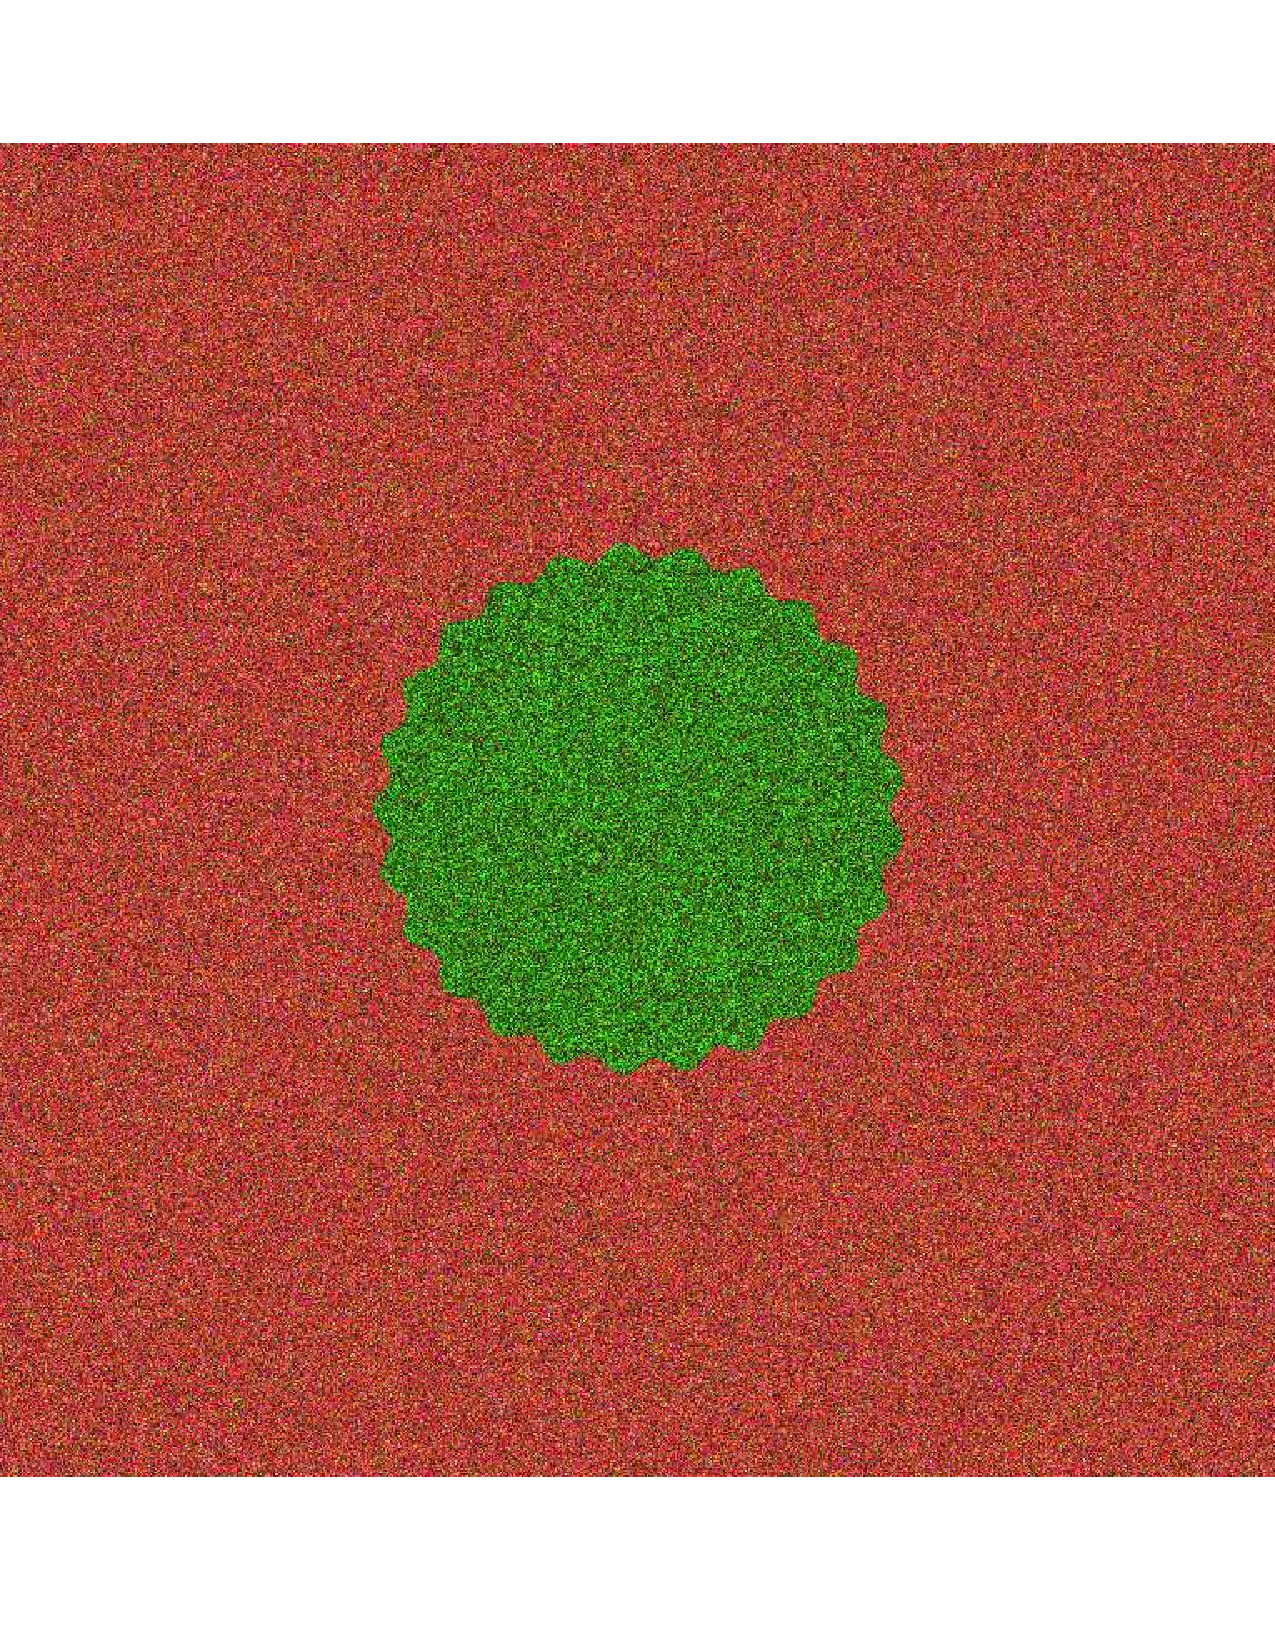
\includegraphics[scale=0.25]{flor_25_155_5_pauli.pdf}}
	\caption{Imagem flor simulada com $\beta = 25$, $\delta = 155$ e $\nu = 5$ .}
\end{figure}
\end{frame}

\begin{frame}{Resultados numéricos}
\begin{figure}[hbt]
\minipage{0.45\textwidth}
	\fbox{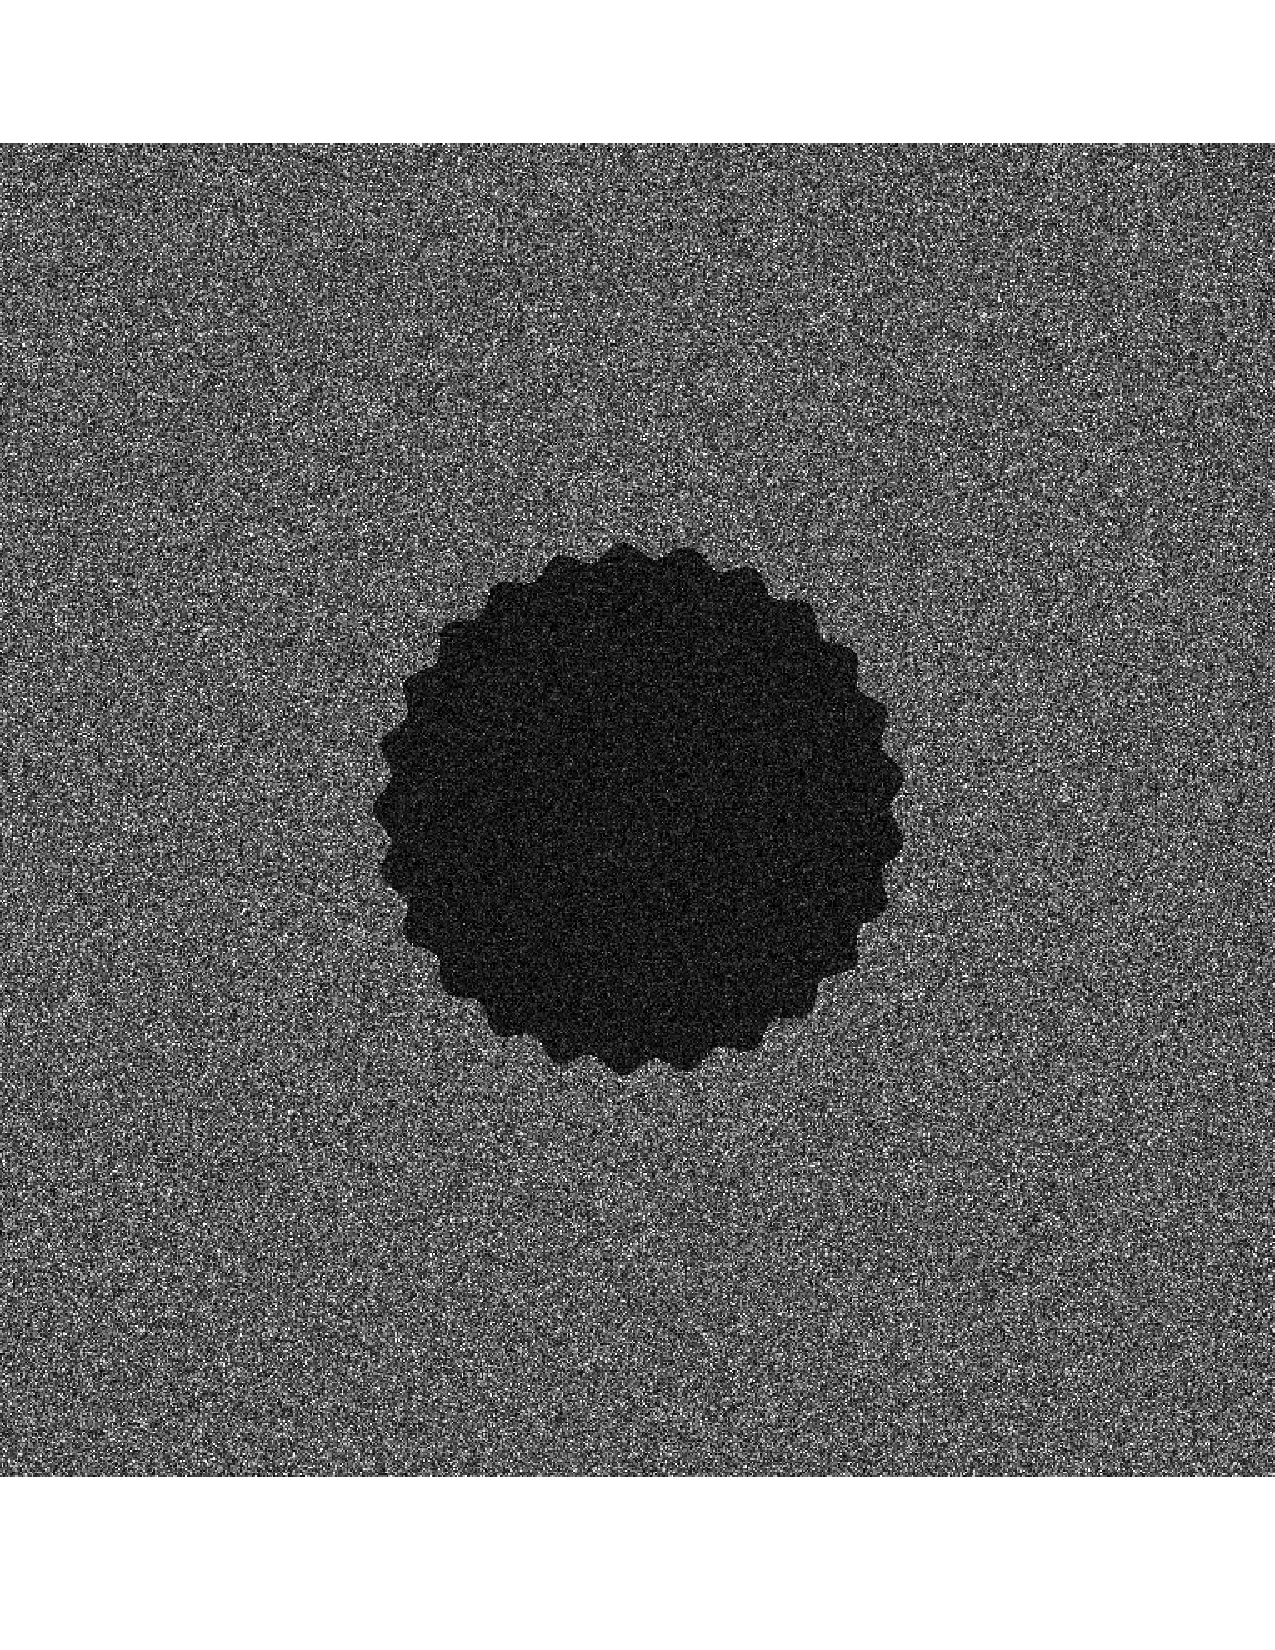
\includegraphics[width=\linewidth]{flor_25_155_5_hh.pdf}}
	\caption{Imagem flor simulada canal $hh$ com $\beta = 25$, $\delta = 155$ e $\nu = 5$ .}
\endminipage\hfill
\minipage{0.45\textwidth}
	\fbox{
\includegraphics[width=\linewidth]{flor_evid_25_155_5_hh.pdf}}
	\caption{Evidências de bordas canal $hh$ com $\beta = 25$, $\delta = 155$ e $\nu = 5$ .}
\endminipage\hfill
\end{figure}
\end{frame}
\begin{frame}{Resultados numéricos}
\begin{figure}[hbt]
\minipage{0.45\textwidth}
	\fbox{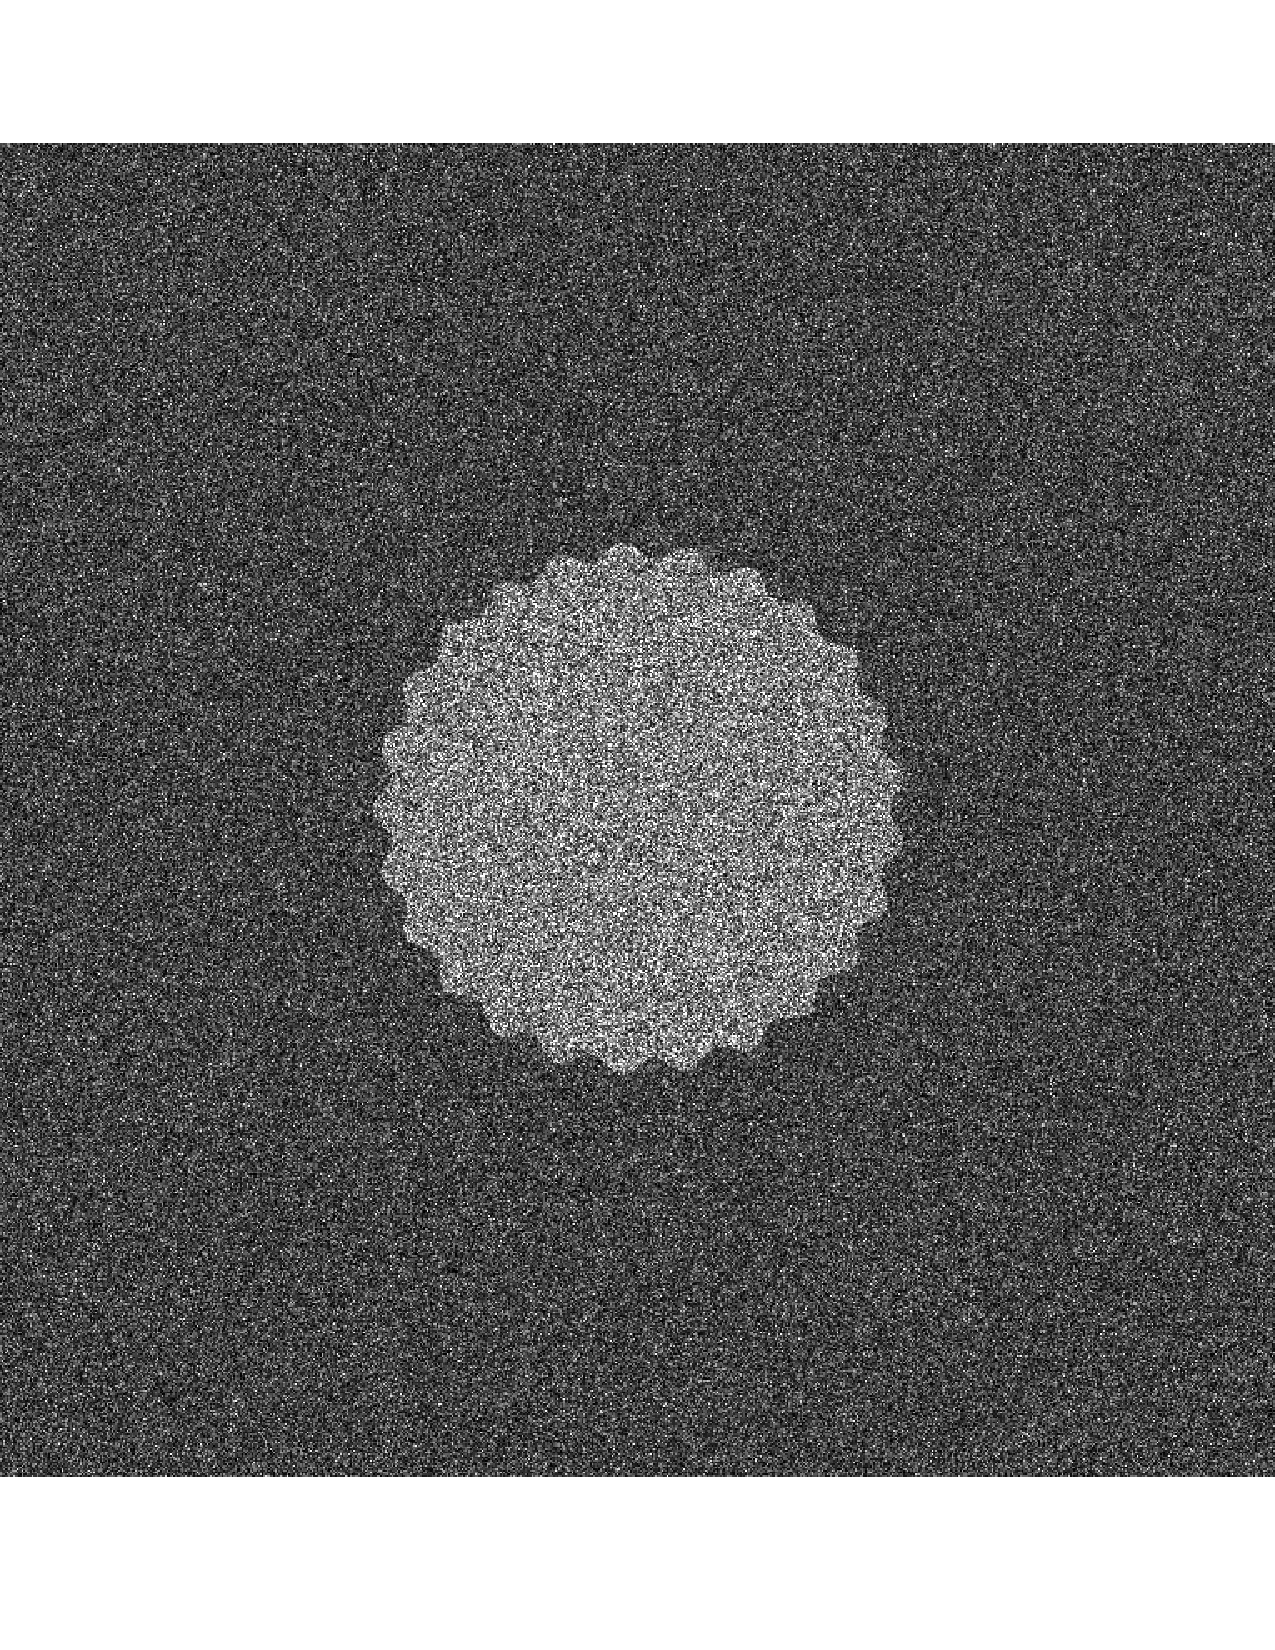
\includegraphics[width=\linewidth]{flor_25_155_5_hv.pdf}}
	\caption{Imagem flor simulada canal $hv$ com $\beta = 25$, $\delta = 155$ e $\nu = 5$ .}
\endminipage\hfill
\minipage{0.45\textwidth}
	\fbox{
\includegraphics[width=\linewidth]{flor_evid_25_155_5_hv.pdf}}
	\caption{Evidências de bordas canal $hv$ com $\beta = 25$, $\delta = 155$ e $\nu = 5$ .}
\endminipage\hfill
\end{figure}
\end{frame}
\begin{frame}{Resultados numéricos}
\begin{figure}[hbt]
\minipage{0.45\textwidth}
	\fbox{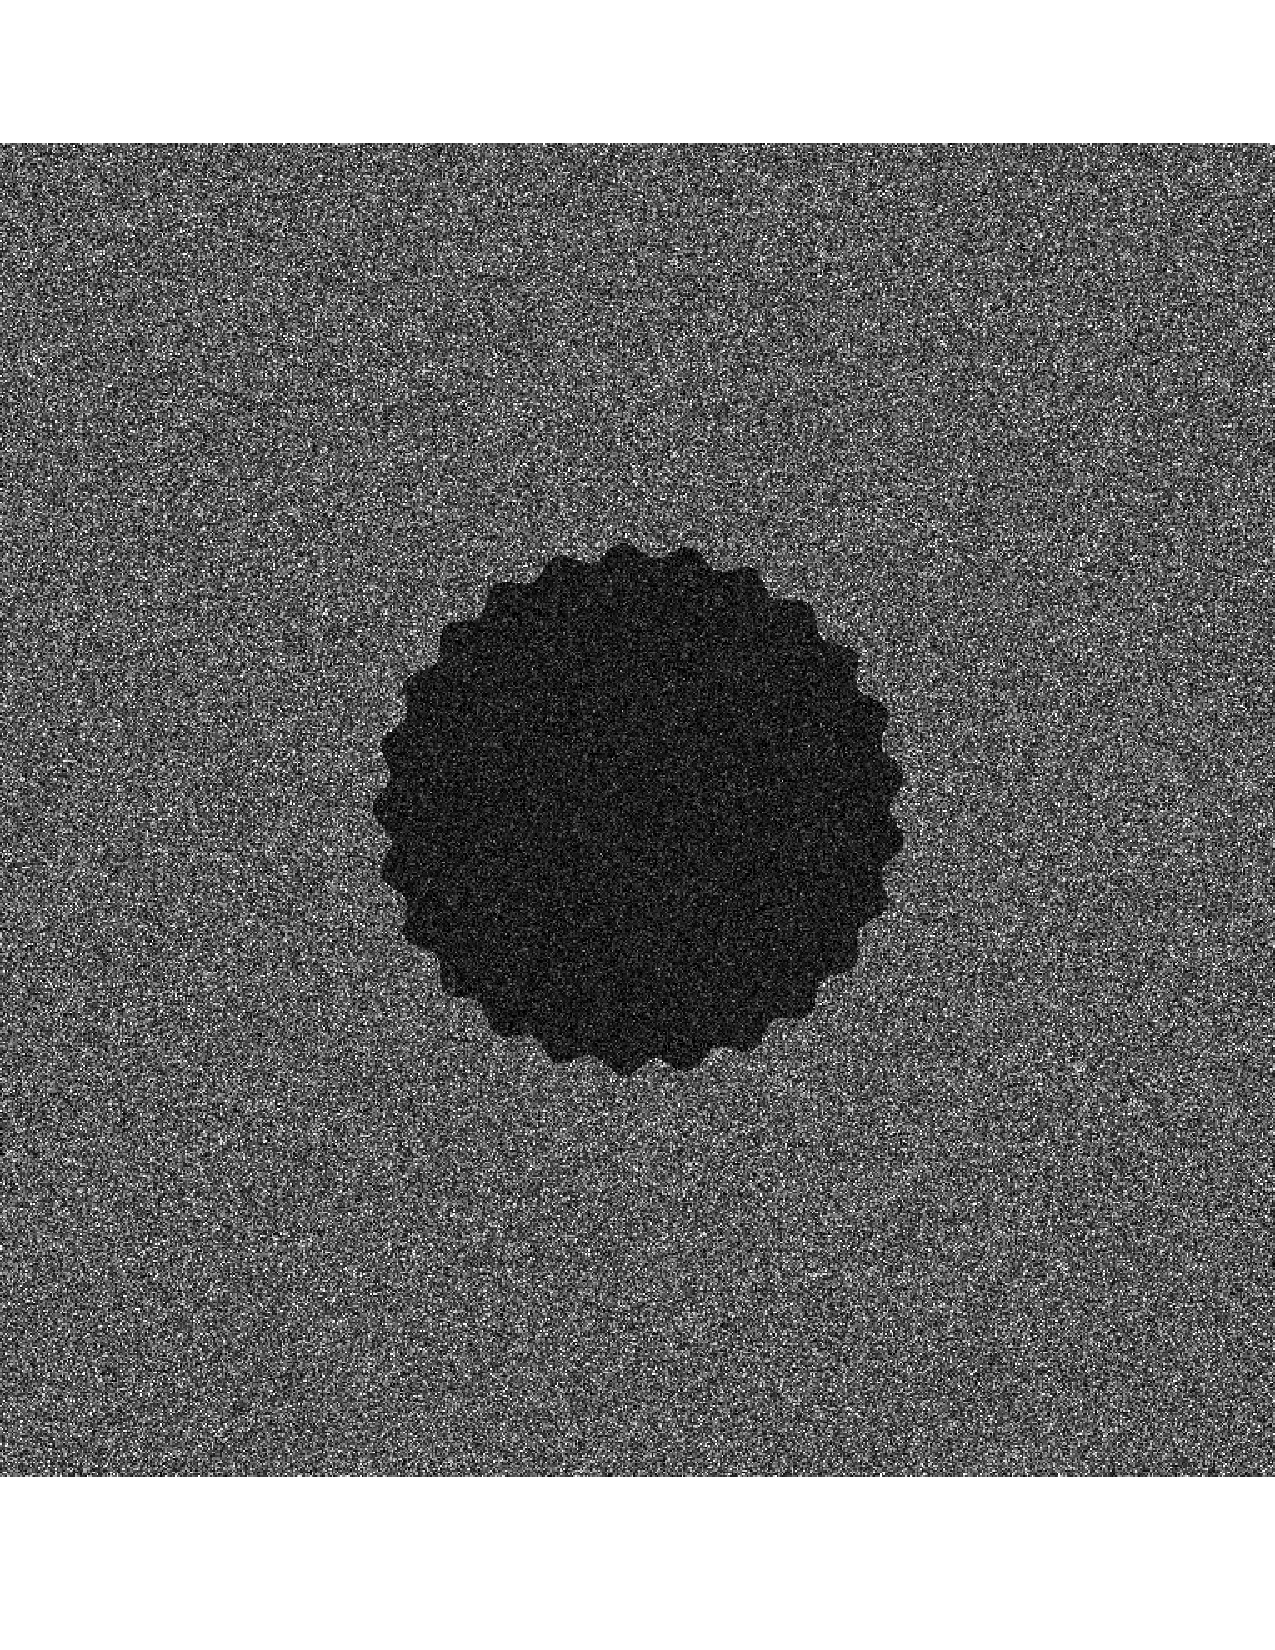
\includegraphics[width=\linewidth]{flor_25_155_5_vv.pdf}}
	\caption{Imagem flor simulada canal $vv$ com $\beta = 25$, $\delta = 155$ e $\nu = 5$ .}
\endminipage\hfill
\minipage{0.45\textwidth}
	\fbox{
\includegraphics[width=\linewidth]{flor_evid_25_155_5_vv.pdf}}
	\caption{Evidencias de bordas canal $vv$ com $\beta = 25$, $\delta = 155$ e $\nu = 5$ .}
\endminipage\hfill
\end{figure}

\end{frame}

\section{Conclusão e trabalhos futuros}

\begin{frame}{Conclusão e trabalhos futuros}
\begin{alertblock}{Conclusão e trabalhos futuros}
\begin{itemize}
\item O método proposto mostrou ser eficiente na detecção de bordas com fusão de evidências;
\item Aplicar o método nas imagens simuladas;
\item Melhorar o método de fusão de evidências de bordas;
	\begin{itemize}
    \item Fusão baseada em histograma, \cite{fbgm};
	\item SVM, Gradient Boosting \cite{ggvlsw};
	\item Randon Forest, \cite{sglmla};
	\item PCA, \cite{mit};
	\item Análises estatísticas, \cite{gs};
	\item Cadeia de Markov com razão de falso alarme constante (CFAR), \cite{flla};
	\item Holistically-Nested Edge Detection \cite{xstz}.
	\end{itemize}
\item Aplicar em imagens reais.
\end{itemize}
\end{alertblock}
\end{frame}

\begin{frame}[standout]
  email: anderborba@gmail.com\\
  Obrigado!!!!
\end{frame}
\begin{frame}[allowframebreaks]
%\bibliographystyle{alpha}
\bibliographystyle{apalike}
\tiny \bibliography{../bibliografia}
\end{frame}

\end{document}
